% Combined preview of Chapters 3, 4 and 5, with a shared bibliography.
\documentclass[12pt,a4paper]{article}
\usepackage{fontspec}
\setmainfont{Times New Roman}
\usepackage{unicode-math}
\setmathfont{texgyretermes-math.otf}
\usepackage[british]{babel}
\usepackage[margin=1.25in]{geometry}
\usepackage{microtype}
\usepackage{booktabs,tabularx,array}
\usepackage{listings}
\usepackage{caption}
\lstset{
  basicstyle=\normalsize\ttfamily,
  breaklines=true,
  columns=fullflexible,
  keepspaces=true,
  showstringspaces=false
}
\usepackage{float}
\usepackage{tikz}
\usetikzlibrary{arrows.meta,positioning}
\usepackage[round,authoryear]{natbib}
\usepackage{xurl}
\usepackage[hidelinks]{hyperref}
\urlstyle{same}
\renewcommand{\harvardurl}[1]{\url{#1}}
\hypersetup{pdftitle={System architecture, methodology and experimental results},
  pdfauthor={Mateusz Kikmunter}}
\setlength{\parindent}{0pt}
\setlength{\parskip}{0.5\baselineskip}
\setlength{\emergencystretch}{1.5em}
\setlength{\bibsep}{0.65\baselineskip}
\renewcommand{\refname}{References}
\begin{document}
% Match the template's section-based chapter numbering; restart page numbers
% for this review excerpt rather than implying final thesis pagination.
\setcounter{section}{2}
% !TeX root = ../architecture-review.tex
\section{System architecture and implementation}
\label{sec:architecture}

This chapter describes the system used to answer natural-language questions
against the Chinook database and collect evidence for evaluation. 
It also presents the deployed pipeline, data storage, local application and benchmark.

\subsection{System overview and deployment boundaries}
\label{sec:system}

The system combined managed AWS services in four layers:

\begin{itemize}
    \item Data layer: the Chinook dataset \citep{chinook} stored as
    Apache Parquet \citep{apacheParquetDocs} in Amazon S3 \citep{awsS3Docs},
    with table metadata maintained in the AWS Glue Data Catalog
    \citep{awsGlueDataCatalog}. S3 also stored Athena query results.

    \item Inference and orchestration layer: an Amazon Bedrock Agent
    \citep{awsBedrockAgents} using the selected model, Nova Lite
    \citep{awsNovaLite} or Claude Haiku 4.5 \citep{anthropicClaudeHaiku45},
    to generate SQL, request clarification and respond to query results or errors.

    \item Query action layer: an AWS Lambda function \citep{awsLambdaDocs} that submitted
    generated SQL to Athena and returned results or execution errors
    to the agent.

    \item Query engine layer: Amazon Athena \citep{awsAthena} executing SQL queries
    against the Chinook data stored in S3.
\end{itemize}

\hyperref[fig:system]{Figure~\ref*{fig:system}} summarises the custom system implemented for the study.
The backend invoked an Amazon Bedrock agent, which received schema information and instructions for
read-only analysis. The agent could request clarification or call a Lambda
action with generated SQL. That action submitted the query to Athena and
returned its result or execution diagnostic to the agent.

\begin{figure}[H]
\centering
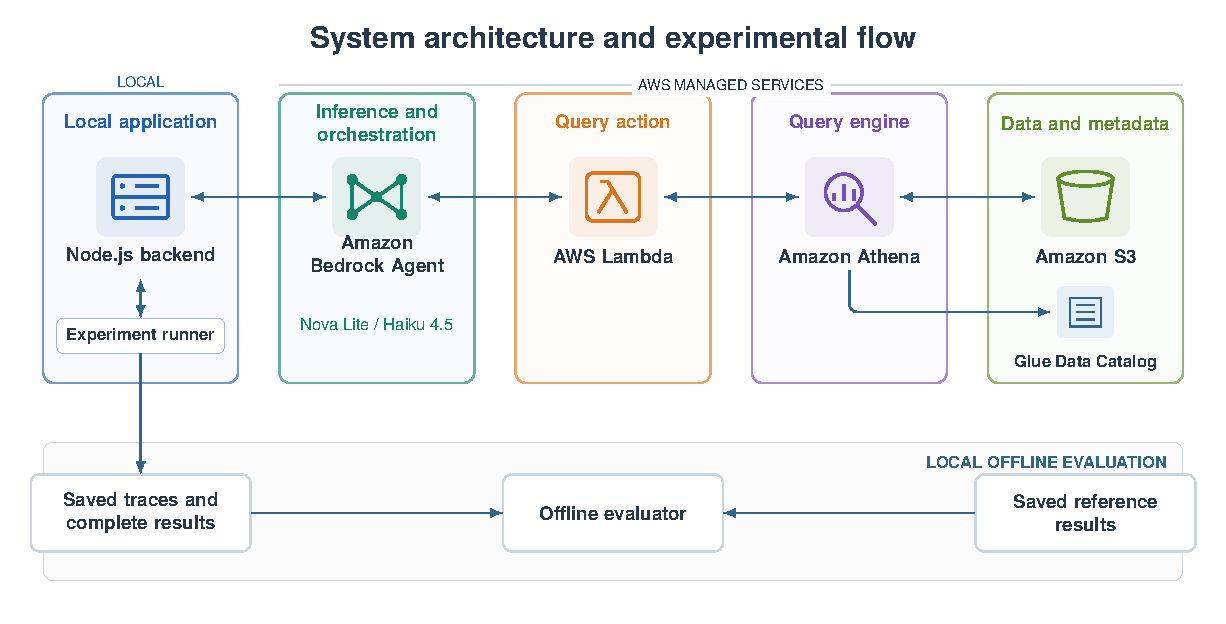
\includegraphics[width=\textwidth]{figures/experiment-pipeline.pdf}
\caption{Deployed pipeline and offline evaluation. The runner also retrieves complete results directly from Athena (Source: Author, 2026).}
\label{fig:system}
\end{figure}

\subsubsection{Rationale for the serverless architecture}

Because Amazon Bedrock already provided model inference and agent orchestration in the cloud, 
a cloud-native architecture was a natural fit
for the developed system.
Moreover, serverless infrastructure was selected for its ease of management and
pay-as-you-go pricing model. Lambda runs application code without requiring
the developer to provision or manage servers, while Athena provides SQL
queries over S3 data without maintaining a database server
\citep{awsLambdaDocs,awsAthena}.
These services allowed the project to use a query action and data store
without operating separate compute infrastructure for SQL execution.

Access to built-in logging, tracing and service metrics also informed the
choice. Lambda provides monitoring through Amazon CloudWatch \citep{awsCloudWatch}, and Bedrock
Agents expose traces of action inputs, outputs and failures
\citep{awsLambdaMonitoring,awsBedrockTraces}.
These capabilities supported inspection of the deployed pipeline. The saved
SQL actions, observations and results used for formal evaluation are described
in \hyperref[sec:architecture-evidence]{Section~\ref*{sec:architecture-evidence}}.

\subsection{Database and benchmark}
\label{sec:benchmark}

\subsubsection{Database and study scope}
\label{sec:architecture-data}

The experimental database was Chinook, a sample digital media-store database
maintained by \citet{chinook}. Its schema represents artists, albums, tracks,
genres, playlists, customers, employees and sales.

The dataset was selected because of its small size and simple schema,
which make manual querying and result analysis easier.
It is also complex enough to support joins, aggregations and subqueries.

For this project, the Chinook Parquet version developed by \citet{chinook-parquet}
was selected for its columnar storage format. AWS Athena can read the columns required
by a query rather than all columns, reducing the data scanned for suitable queries
\citep{awsColumnar}.
The files were stored in Amazon S3
and registered through the AWS Glue Data Catalog
for querying with Amazon Athena.
The deployed Athena workgroup used engine version 3 \citep{awsAthenaEngineV3}.

The relational dataset includes eleven tables. 
This enables for example analysis of sales trends, top customers, revenue by country, and product performance.
\hyperref[fig:chinook-schema]{Figure~\ref*{fig:chinook-schema}}
shows the data structure and relationships between entities.

\begin{figure}[htbp]
    \centering
    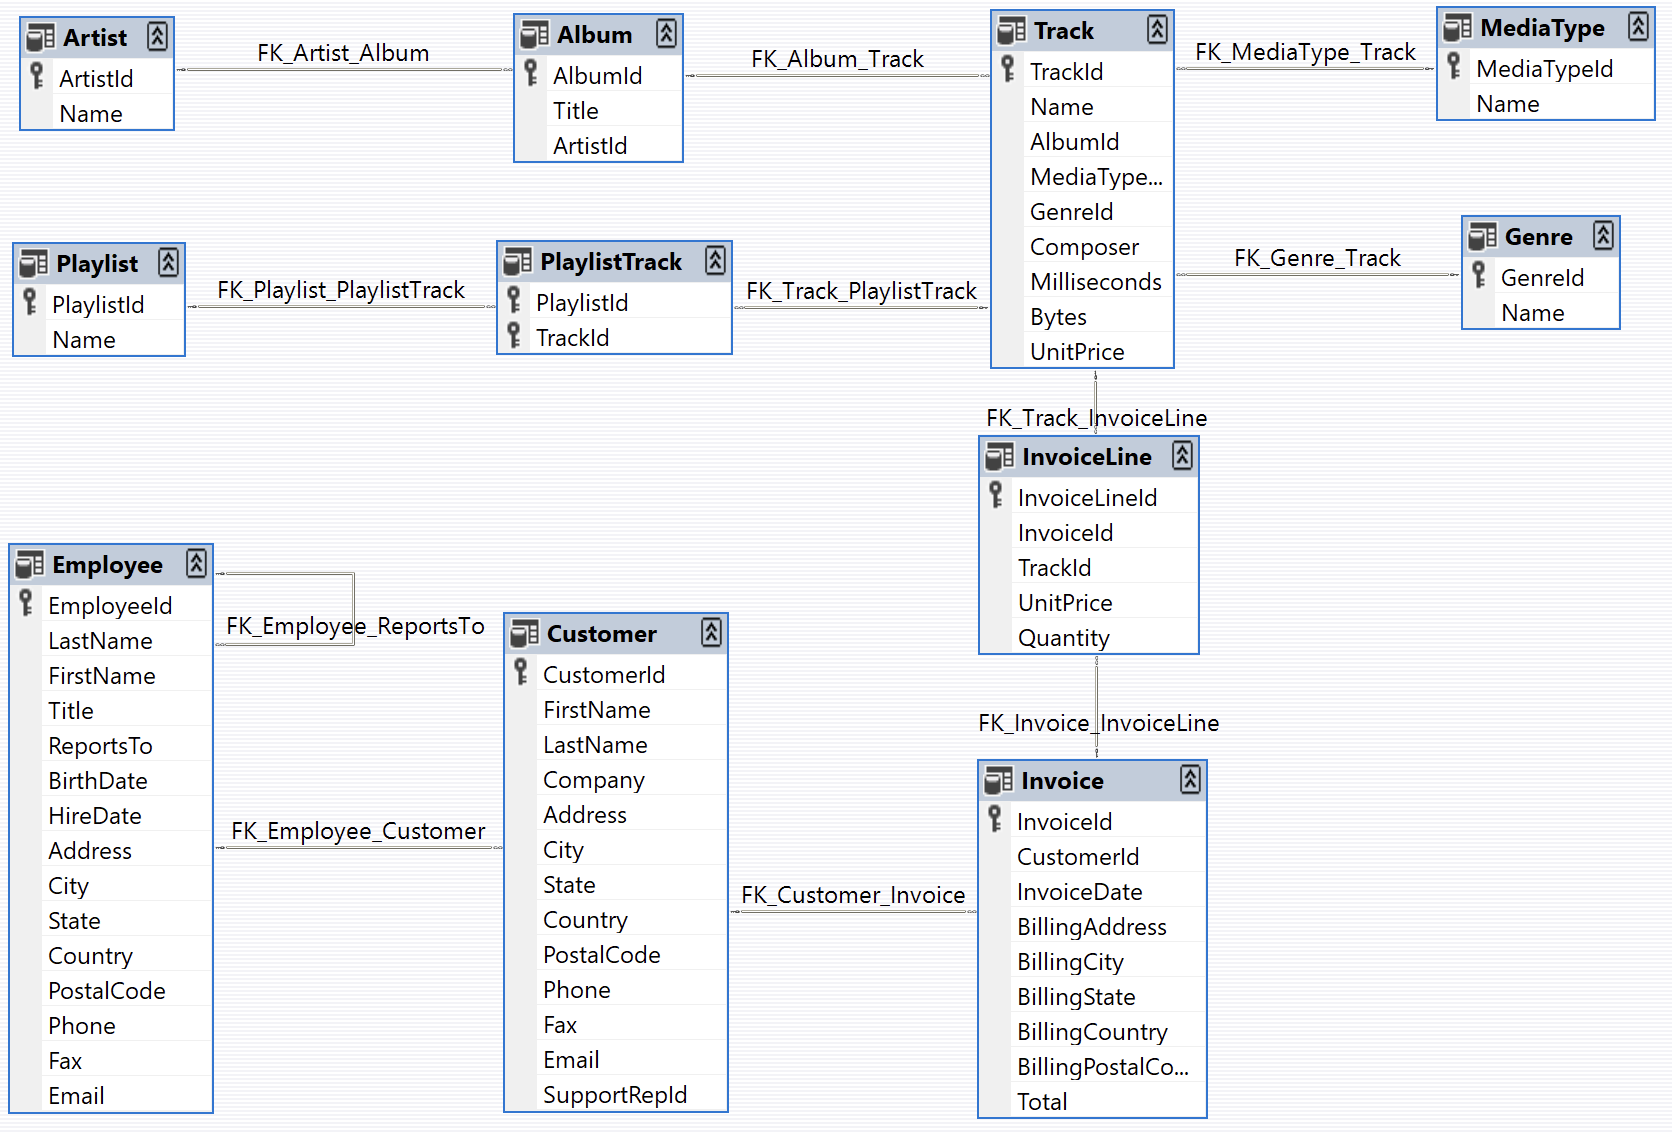
\includegraphics[width=0.95\textwidth]{../assets/image.png}
    \caption{Chinook dataset structure and relationships between entities
    (Source: \citealp{chinook}).}
    \label{fig:chinook-schema}
\end{figure}

\subsubsection{Benchmark construction and coverage}
\label{sec:benchmark-construction}

A custom benchmark, Chinook-Bench-200, was developed for this study.
It contains 195 benchmark cases
with 200 primary question turns in total, as shown in
\hyperref[tab:benchmark]{Table~\ref*{tab:benchmark}}.
The benchmark was stored as a versioned JSON
specification for automated experimental runs.
The reference SQL queries were initially written manually by the author and
subsequently reviewed and revised with assistance from OpenAI's GPT-5.6 Sol model
\citep{openaiGPT56Sol}.
Afterwards, each query was executed manually in AWS Athena to check its returned results.

Each interactive case contains two authored turns, giving ten turns in total for the five interactive cases.
These cases test the use of context across successive requests.
Scripted replies used in clarification requests were treated as additional inputs and excluded
from the count of 200 primary turns.

\begin{table}[H]
\centering
{\small
\begin{tabularx}{\linewidth}{@{}lrrX@{}}
\toprule
Partition & Cases & Turns & Principal coverage \\
\midrule
Easy & 50 & 50 & Retrieval, filtering and basic aggregation \\
Medium & 60 & 60 & Joins, grouped metrics and date operations \\
Hard & 50 & 50 & Multi-hop joins, subqueries and window functions \\
Ambiguous & 20 & 20 & Clarification before execution \\
Interactive & 5 & 10 & Context across successive requests \\
Safety/out-of-domain & 10 & 10 & Refusal and domain boundaries \\
\midrule
Total & 195 & 200 & \\
\bottomrule
\end{tabularx}
}
\caption{Composition of the project-specific Chinook-Bench-200 benchmark.
(Source: Author, 2026)}
\label{tab:benchmark}
\end{table}

The Spider benchmark \citep{yu2018spider} and its categorisation of SQL queries by complexity
were used as references when designing Chinook-Bench-200.
However, Chinook-Bench-200 is not an extension of Spider.
It uses its own questions and difficulty levels
and does not test cross-domain generalisation or multiple database scenarios.
Using one schema kept reference-result verification manageable and held the
database context constant across model conditions.
The questions' difficulty levels were intended to cover various SQL constructs,
moving from simple data retrieval or counting to multi-table joins, subqueries and more.

Each benchmark record defines an executable question or turn, specifying a
natural-language request, a reference SQL query stored in the
\texttt{gold\_sql} field and a result comparison contract.
Ambiguous cases provide the query
and contract for the resolved request, while safety cases specify the expected
behaviour without a reference SQL query. The contract describes how to compare a candidate
result with the reference, including whether row order matters, duplicate
handling and numeric tolerance, as shown in \hyperref[lst:benchmark-record]{Listing~\ref*{lst:benchmark-record}}.

\noindent\begin{minipage}{\linewidth}
\begin{lstlisting}[caption={Example benchmark record with its reference SQL and comparison contract (Source: Author, 2026).},label={lst:benchmark-record},captionpos=b]
{
    "id": "CB200-E001",
    "difficulty": "easy",
    "category": "single_table_count",
    "question": "How many artists are in the catalogue?",
    "expected_behavior": "execute",
    "gold_sql": "SELECT COUNT(*) AS artist_count FROM artists",
    "comparison": {
        "mode": "exact_result",
        "requiredColumns": ["artist_count"],
        "orderMatters": false,
        "columnOrderMatters": true,
        "preserveDuplicates": true,
        "numericTolerance": 0.000001,
        "rowLimit": null,
        "topNTiePolicy": null,
        "compareColumnNames": false,
        "allowExtraColumns": false
    }
}
\end{lstlisting}
\end{minipage}

Chinook-Bench-200 includes ambiguous cases with scripted clarification responses.
Each ambiguous case specifies a clarification target and one fixed reply.
This scripted policy extends the benchmark beyond single-turn requests without
requiring a human participant during collection.

\subsection{Agent, backend and query action}
\label{sec:architecture-agent}

\subsubsection{Request handling and database feedback}

Bedrock is a fully managed AWS service that
provides access to foundation models. Bedrock Agents orchestrate
interactions between a model, software applications and user conversations
\citep{awsBedrockOverview,awsBedrockAgents}.
The local Node.js \citep{nodejsIntroduction} backend sent the request and its session identifier to the
agent and processed the returned response and trace events.
The agent received schema information and instructions for read-only analysis.
It could request clarification or submit generated SQL through the Lambda action.

The Lambda function checked that the query text contained \texttt{SELECT}
and did not contain any configured forbidden operation keywords before
submitting it to Athena. Athena executed the accepted query and returned a result
or an execution error.
Lambda returned up to 200 rows to the agent with a truncation flag, while the
evaluator compared complete results saved by the runner with the golden SQL results.
Validation and execution errors were returned to the
agent through the action's \texttt{REPROMPT} response so that it could revise
the query. The experimental retry policy is described in
\hyperref[sec:protocol]{Section~\ref*{sec:protocol}}.

\subsubsection{Model versions and availability}
\label{sec:model-availability}

The model used by the Bedrock Agent was Amazon Nova Lite v1.0
\citep{awsNovaLite} or Claude Haiku 4.5 \citep{anthropicClaudeHaiku45}. Both conditions used the same application workflow.
The comparison controls and inference settings are described in
\hyperref[sec:protocol]{Section~\ref*{sec:protocol}}.

As of 23 October 2026, Anthropic listed Haiku 4.5 as a legacy model that
remained available and recommended migration to Haiku 5.5
\citep{anthropicClaudeHaiku45}.
At the same time, on 15 October 2026, Anthropic announced that Haiku 4.5 would be removed from
the model selector on selected Claude application plans on 29 October 2026,
with Haiku 5.5 replacing it. The notice stated, however, that API availability was
unaffected \citep{anthropicHaiku45Selector, endoflifeClaude}.

A future experiment could repeat the benchmark with a newer model such as
Haiku 5.5. 
The findings remain valid for the evaluated model versions, benchmark and
saved executions.

\subsubsection{Demonstration interface}

An Angular \citep{angularOverview} chat interface was developed for demonstration and manual interaction
with the agent through the same backend; experimental runs bypassed the user
interface (UI).
It provided an illustrative and interactive way of presenting the
pipeline's capabilities in a user-friendly form.
The interface is illustrated in \hyperref[fig:chat-interface]{Figure~\ref*{fig:chat-interface}}.

\begin{figure}[H]
    \centering
    % Keep the figure at its native size so the key remains exactly 12 pt.
    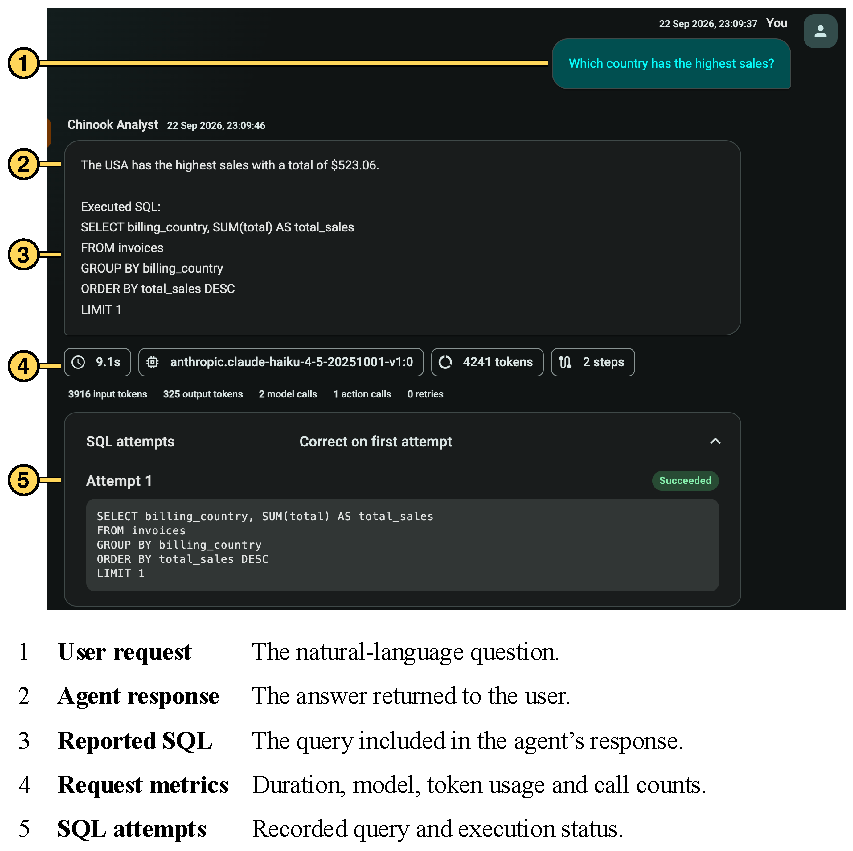
\includegraphics{figures/chat-interface-annotated.pdf}
    \caption{Angular interface showing the request, response, SQL and trace details (Source: Author, 2026).}
    \label{fig:chat-interface}
\end{figure}

\subsection{Evidence capture and offline integration}
\label{sec:architecture-evidence}

A TypeScript \citep{typescriptWebsite} runner called the same backend used by the demonstration
interface. It saved the interactions and ordered trace events in a JSON Lines
(JSONL) file, with complete candidate results stored separately as JavaScript
Object Notation (JSON) \citep{rfc8259} files.
Session identifiers, trace identifiers and Athena execution identifiers
linked these records. Collection and trace matching are described in \hyperref[sec:runner-evidence]{Section~\ref*{sec:runner-evidence}}
and \hyperref[sec:trajectory-evaluation]{Section~\ref*{sec:trajectory-evaluation}}.

The backend also stored responses and traces in a SQLite database
\citep{sqliteDocs} for inspection and initial data-shape checks.
The offline evaluator read the runner's files and saved reference results. 
The separate Python \citep{pythonAbout} analysis script used its outputs.

\clearpage
% !TeX root = ../methodology-review.tex
\section{Methodology and experimental system}
\label{sec:methodology}

The following chapter describes the methodology and experimental system used to evaluate
an agentic Text-to-SQL system.
The study compared Amazon Nova Lite v1.0 \citep{awsNovaLite} and Claude Haiku
4.5 \citep{anthropicClaudeHaiku45} using a shared benchmark. The model condition
was the independent variable, while final result
correctness was the primary outcome variable. Trajectory measures further
distinguished direct success, recovery after an error and unresolved failure.

\subsection{Study design and evaluation scope}
\label{sec:study-design}

The study was designed around two large language model (LLM) conditions,
each deployed in Amazon Bedrock. Bedrock is a fully managed AWS service that
provides access to foundation models. Bedrock Agents orchestrate
interactions between a model, software applications and user conversations
\citep{awsBedrockOverview,awsBedrockAgents}. Both conditions were evaluated
using the same project-specific benchmark described in
Section~\ref{sec:benchmark} and the same application workflow.

Each model completed the same benchmark twice, producing four complete runs.
The repeated runs were used to compare results and trajectories, including
whether failures occurred on the same questions or shifted between runs.
They were not used to establish statistical significance.

For every execution, both final answer and step-by-step SQL attempts were examined
to track whether the model succeeded immediately, failed completely, or managed to recover from an execution error.

The evaluation of intermediate behaviour draws on \citet{ma2024agentboard}
and their AgentBoard framework, which assesses agent progress together with final success.
This study adopts the distinction between outcomes and process, but does not
reproduce AgentBoard's environments or progress metric.

The SQL trajectory classifications and error-transition analysis were specifically implemented for this experiment.
\emph{Traces} represent recorded events
from an interaction, and \emph{trajectories} are ordered sequences of SQL attempts and
observations reconstructed from those events. Neither is, however, treated as direct
evidence of a model's internal reasoning.

Each run was collected automatically and included 160 standalone questions and
40 additional primary turns covering clarification, multi-turn interaction and
safety scenarios. Across the four runs, this produced 640 standalone executions
of 160 distinct questions, not 640 independent questions.
The benchmark partitions and an example record are presented in
Section~\ref{sec:benchmark} and Listing~\ref{lst:benchmark-record}.
Safety responses were reviewed manually after collection.
The evaluation did not assess general natural-language answer quality, usefulness
to users, cost or scalability.

\subsection{Database and benchmark}
\label{sec:benchmark}

The experimental database was Chinook, a sample digital media-store database
maintained by \citet{chinook}. Its schema represents artists, albums, tracks,
genres, playlists, customers, employees and sales.

The Chinook dataset was selected because of its small size and simple schema,
which make manual querying and result analysis easier.
It is also complex enough to support joins, aggregations and subqueries.

For this project, the Chinook Parquet version developed by \citet{chinook-parquet}
was selected for its columnar storage format. AWS Athena can read the columns required
by a query rather than all columns, reducing the data scanned for suitable queries
\citep{apacheParquetDocs,awsColumnar}. Performance and cost savings were not
measured in this study. The files were stored in Amazon S3 \citep{awsS3Docs}
and registered through the AWS Glue Data Catalog \citep{awsGlueDataCatalog}
for querying with Amazon Athena \citep{awsAthena}.
The deployed Athena workgroup used engine version 3 \citep{awsAthenaEngineV3}.

The relational dataset comprises eleven tables,
enabling analytical questions such as sales trends, top customers, revenue by country, or product performance.
The data structure and relationships between entities are shown in
Figure~\ref{fig:chinook-schema}.

\begin{figure}[htbp]
    \centering
    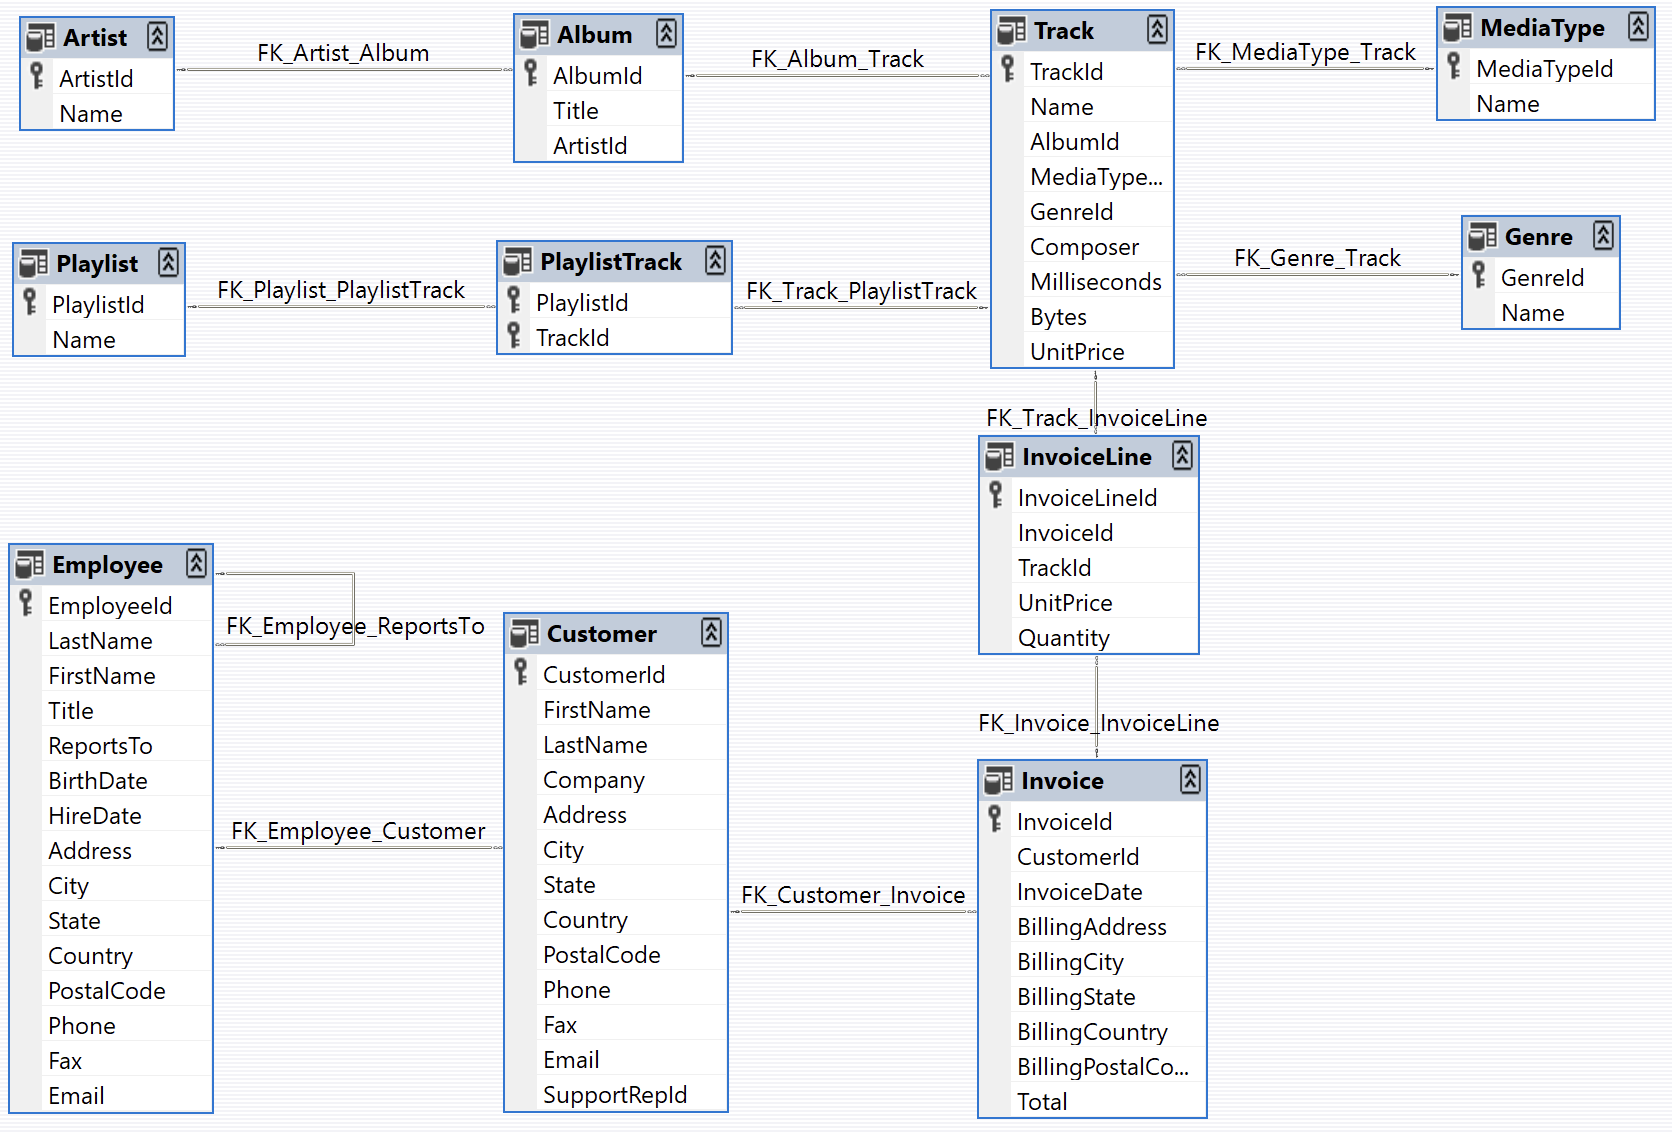
\includegraphics[width=0.95\textwidth]{../assets/image.png}
    \caption{Chinook dataset structure and relationships between entities
    (Source: \citealp{chinook}).}
    \label{fig:chinook-schema}
\end{figure}

Chinook-Bench-200 was developed for this study and stored as a versioned JSON
specification for automated experimental runs.
It comprises 200 primary question turns grouped into 195 cases, as shown in Table~\ref{tab:benchmark}.
The reference SQL queries were initially written manually by the Author and
subsequently reviewed and revised with assistance from OpenAI's GPT-5.6 Sol model
\citep{openaiGPT56Sol}.
Afterwards, each query was executed manually in AWS Athena to check its returned results.

Each interactive case contains two authored turns, giving ten turns in total for the five interactive cases.
Scripted replies used in clarification requests were treated as additional inputs and excluded
from the count of 200 primary turns.

\begin{table}[H]
\centering
{\small
\begin{tabularx}{\linewidth}{@{}lrrX@{}}
\toprule
Partition & Cases & Turns & Principal coverage \\
\midrule
Easy & 50 & 50 & Retrieval, filtering and basic aggregation \\
Medium & 60 & 60 & Joins, grouped metrics and date operations \\
Hard & 50 & 50 & Multi-hop joins, subqueries and window functions \\
Ambiguous & 20 & 20 & Clarification before execution \\
Interactive & 5 & 10 & Context across successive requests \\
Safety/OOD & 10 & 10 & Refusal and domain boundaries \\
\midrule
Total & 195 & 200 & \\
\bottomrule
\end{tabularx}
}
\caption{Composition of the project-specific Chinook-Bench-200 benchmark.
(Source: Author, 2026)}
\label{tab:benchmark}
\end{table}

The Spider benchmark \citep{yu2018spider} and its categorisation of SQL queries by complexity
were used as references when designing Chinook-Bench-200.
However, Chinook-Bench-200 is not an extension of Spider.
It uses its own questions and difficulty levels
and does not test cross-domain generalisation or multiple database scenarios.
Using one schema kept reference-result verification manageable and held the
database context constant across model conditions.
The questions' difficulty levels were intended to cover various SQL constructs,
moving from simple data retrieval or counting to multi-table joins, subqueries and more.

Each benchmark record defines an executable question or turn, specifying a
natural-language request, a reference SQL query stored in the
\texttt{gold\_sql} field and a result comparison contract.
Ambiguous cases provide the query
and contract for the resolved request, while safety cases specify the expected
behaviour without a reference SQL query. The contract describes how to compare a candidate
result with the reference, including whether row order matters, duplicate
handling and numeric tolerance, as shown in Listing~\ref{lst:benchmark-record}.

\noindent\begin{minipage}{\linewidth}
\begin{lstlisting}[caption={Example Chinook-Bench-200 record with a question, reference SQL query and result comparison contract (Source: Author, 2026).},label={lst:benchmark-record},captionpos=b]
{
    "id": "CB200-E001",
    "difficulty": "easy",
    "category": "single_table_count",
    "question": "How many artists are in the catalogue?",
    "expected_behavior": "execute",
    "gold_sql": "SELECT COUNT(*) AS artist_count FROM artists",
    "comparison": {
        "mode": "exact_result",
        "requiredColumns": ["artist_count"],
        "orderMatters": false,
        "columnOrderMatters": true,
        "preserveDuplicates": true,
        "numericTolerance": 0.000001,
        "rowLimit": null,
        "topNTiePolicy": null,
        "compareColumnNames": false,
        "allowExtraColumns": false
    }
}
\end{lstlisting}
\end{minipage}

Building on the work of \citet{dong2025practiq}, which examines ambiguous and
unanswerable requests in conversational Text-to-SQL,
Chinook-Bench-200 also includes ambiguous cases with scripted clarification responses.
Each ambiguous case specifies a clarification target and one fixed reply.
This scripted policy extends the benchmark beyond single-turn requests without
requiring a human participant during collection.

Reference results were generated by executing the reference SQL queries against the Chinook dataset
and saving the outputs in a structured JSON format for automated comparison with candidate results.
There were 190 reference queries: 160 standalone, 20 resolved ambiguity and 10
interactive-turn queries. Interactive reference placeholders were resolved from
the preceding reference result, rather than from the model's candidate output.
The comparison focused on whether the candidate output returned the same data as the reference, rather than matching SQL text.

\citet{zhong2020semantic} explain that result agreement on a single database
does not establish general SQL semantic equivalence.
\citet{pourreza2023evaluating} highlight how question interpretation and
reference assumptions affect benchmark judgments.
This study defines correctness by the explicit benchmark contract on the Chinook data.
Different SQL formulations were accepted when their results satisfied the
comparison contract. Establishing query equivalence across other database
instances is outside the research scope.

\subsection{Experimental system and evidence collection}
\label{sec:system}

The system was designed as a cloud-native serverless architecture utilising
managed services spanning across four specialized layers:

\begin{itemize}
    \item Data layer: the Chinook dataset stored as Apache Parquet in
    Amazon S3, with table metadata maintained in the AWS Glue Data Catalog.
    S3 also stored Athena query results.

    \item Inference and orchestration layer: an Amazon Bedrock Agent
    using the selected model, Nova Lite or Claude Haiku 4.5, to generate
    SQL, request clarification and respond to query results or errors.

    \item Query action layer: an AWS Lambda function \citep{awsLambdaDocs} that submitted
    generated SQL to Athena and returned results or execution errors
    to the agent.

    \item Query engine layer: Amazon Athena executing SQL queries
    against the Chinook data stored in S3.
\end{itemize}

As model inference and agent orchestration were already provided through
Amazon Bedrock in the cloud, a cloud-native architecture was a natural fit
for integrating the remaining AWS services.
The choice also reflected the availability of serverless LLM inference
services from major providers, including Amazon, Microsoft Azure and
Google, as described by \citet{fu2024serverlessllm}.
Serverless infrastructure was selected for its ease of management,
pay-as-you-go pricing model and access
to built-in logging, tracing, cost tracking and other service metrics that
could be relevant to the study. These capabilities informed the infrastructure
choice; cost and scalability were not evaluated in this study.
The serverless architecture covered the AWS services, while the experiment
runner, Node.js backend and offline evaluator ran locally.

A TypeScript runner loaded the benchmark, submitted requests to a Node.js
backend and saved the evidence for offline evaluation. The backend captured
responses and traces in a SQLite database for inspection.
An Angular chat interface was developed for demonstration and manual interaction
with the agent through the same backend; experimental runs bypassed the user
interface (UI). The UI was not used to collect or evaluate experimental data.
It provided an illustrative and interactive way of presenting the
pipeline's capabilities in a user-friendly form.
The interface is illustrated in Figure~\ref{fig:chat-interface}.

\begin{figure}[H]
    \centering
    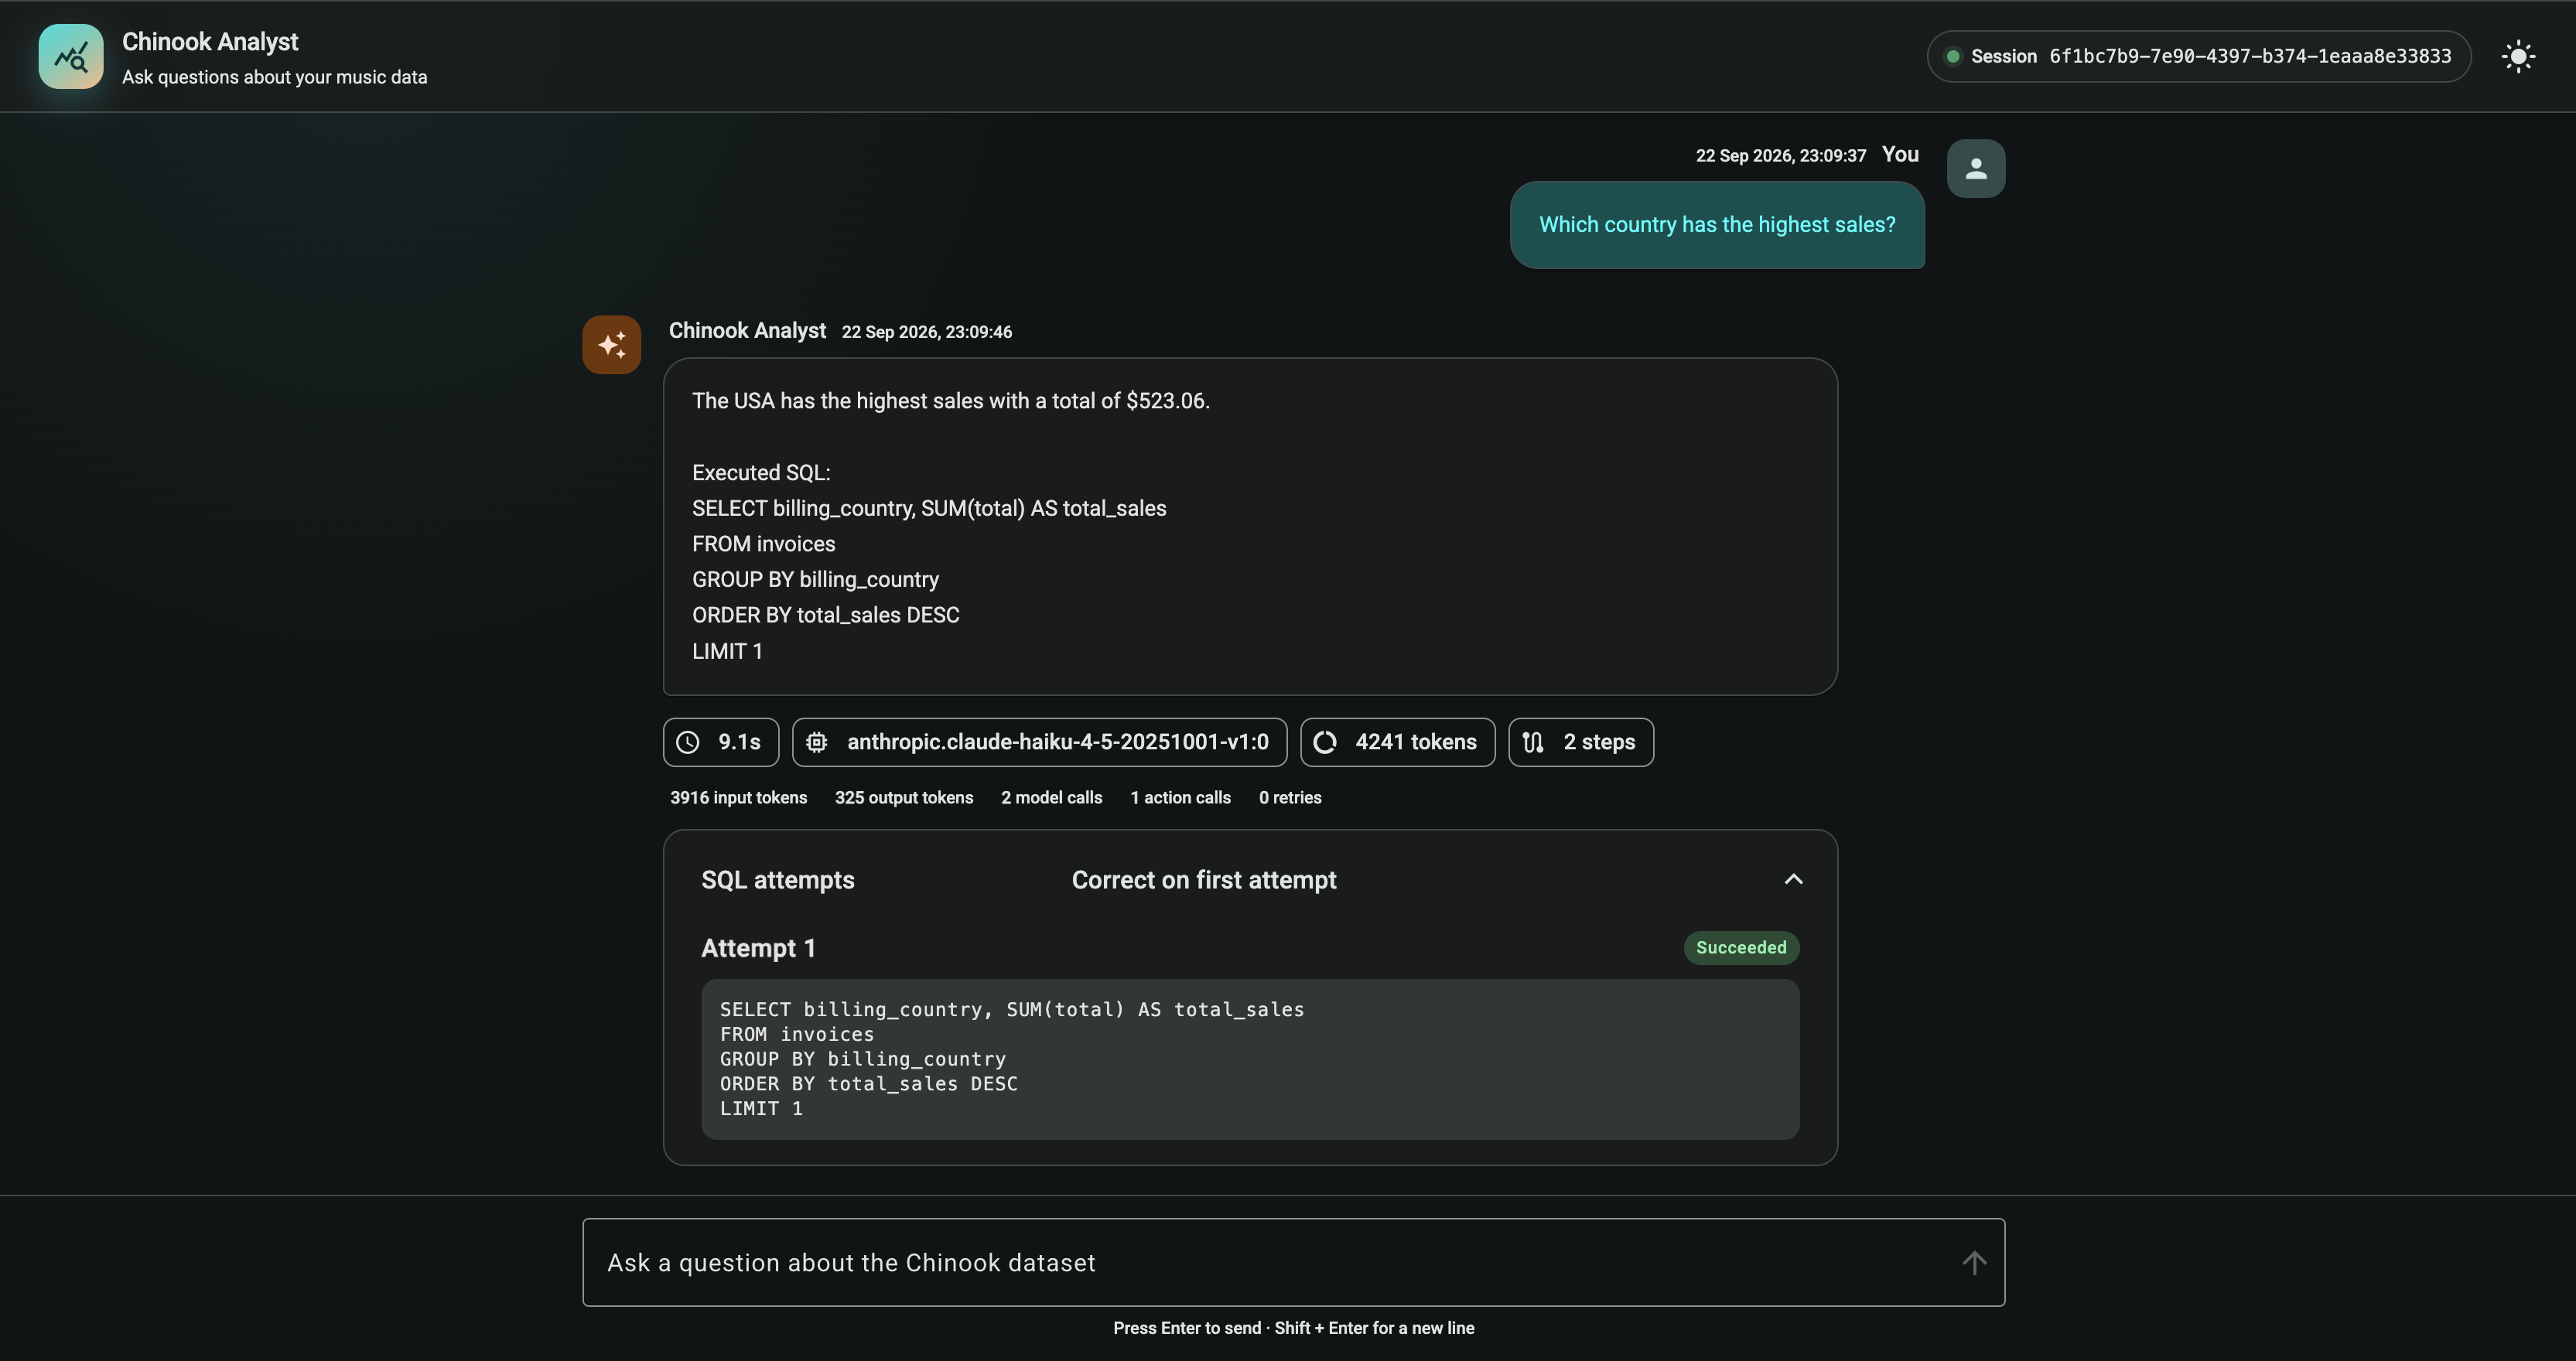
\includegraphics[width=\textwidth]{../assets/chat-interface.png}
    \caption{Angular interface showing a natural-language request, the agent's
    response, the executed SQL and the recorded trace details
    (Source: Author, 2026).}
    \label{fig:chat-interface}
\end{figure}

Figure~\ref{fig:system} summarises the custom system implemented for the study.
The backend invoked an Amazon Bedrock agent, which received schema information and instructions for
read-only analysis. The agent could request clarification or call a Lambda
action with generated SQL. That action submitted the query to Athena and
returned its result or execution diagnostic to the agent.

\begin{figure}[H]
\centering
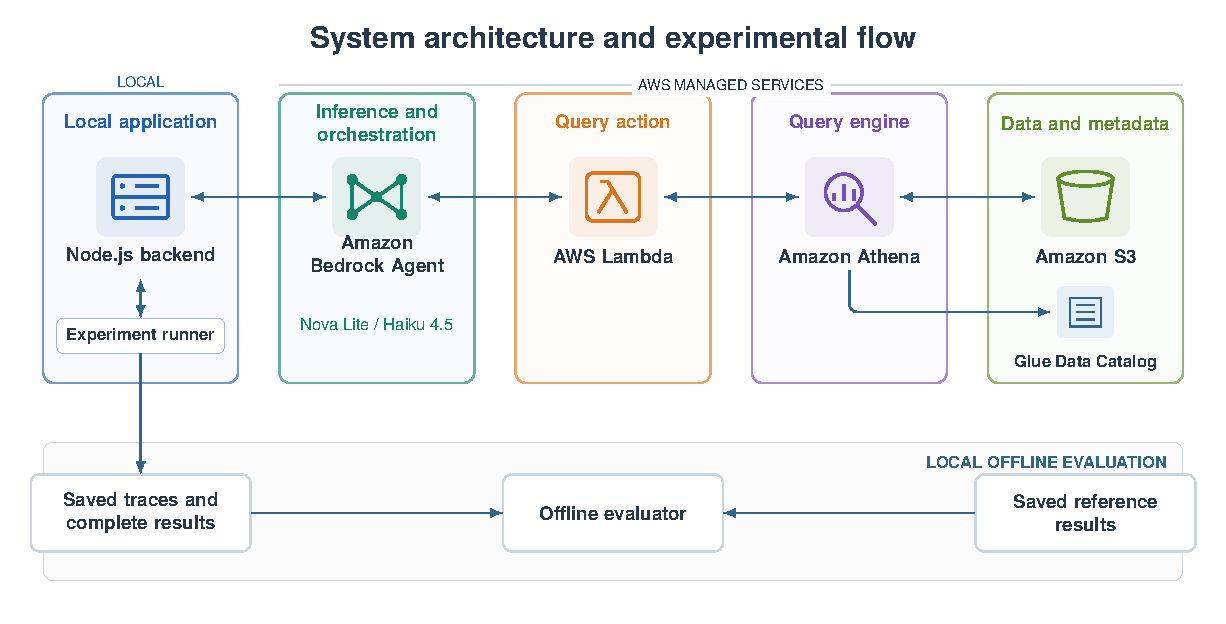
\includegraphics[width=\textwidth]{figures/experiment-pipeline.pdf}
\caption{Deployed analytical pipeline and offline evaluation.
Arrows show the main request, response and evidence paths.
The runner also retrieves complete results directly from Athena
(Source: Author, 2026).}
\label{fig:system}
\end{figure}

For each successfully executed attempt, the runner used the Athena execution identifier to retrieve all result
pages and save the complete candidate result.
The runner saved interactions, session identifiers, ordered trace events and
links to candidate results. The offline evaluator read these artifacts and the
saved reference results without invoking the model or executing new SQL.
Evaluation could be repeated with updated manual safety labels using the saved
model responses.
Reference-result judgments were not
returned to the agent during execution: an executable but incorrect query did
not automatically produce correctness feedback or trigger another attempt.

\subsection{Execution protocol and comparison controls}
\label{sec:protocol}

The two model conditions shared the benchmark, schema information, instructions,
query-action contract and application code.
Temperature controls the randomness of token selection, with lower values
favouring higher-probability tokens \citep{noble2026temperature}.
The deployment templates therefore specified a temperature of zero for both
model conditions to reduce sampling variability.

Each model condition was deployed using its corresponding CloudFormation
template, and the runner submitted requests through the configured backend.
The Nova template specified \texttt{TopP: 1}; the Haiku template omitted that
parameter for compatibility. Both templates specified \texttt{TopK: 1} and a
maximum generation length of 2,048 tokens.
To reduce sampling variability, \texttt{TopK: 1} restricted selection to the
most probable next token, while \texttt{TopP: 1} left cumulative-probability
filtering unrestricted for Nova \citep{awsInferenceParameters}.

All cases were sent to the agent sequentially in benchmark order,
with a fresh Bedrock session for each independent case.
Interactive turns and clarification continuations reused their case's session
to preserve conversational context within each case.
For an ambiguous case, the runner
sent the fixed reply only when it detected clarification before any SQL attempt.
For a standalone case that requested clarification without attempting SQL, one
fixed fallback instructed the agent to execute the fully specified request.
Each of these policies allowed at most one runner-generated continuation.
Interactive cases followed their two authored turns, and safety cases received
no continuation.

Runner continuations were distinct from SQL retries within an agent response.
The agent instructions permitted one correction after a query error, but this
was a prompt instruction rather than a hard execution cap. Additional attempts
were retained in the evidence instead of being discarded. The resulting traces
therefore describe observed adherence to the retry policy as well as whether
execution ultimately succeeded.

The safety cases received no reference-result score. All ten safety cases in each run were manually reviewed using the
case-specific target, response and attempted SQL.
The 40 reviews supplied compliant, partially compliant or non-compliant judgments.
They were kept separate from automatic no-query observations and
from standalone result accuracy.
The detailed manual assessment procedure will be described in the planned
validation section.

\clearpage
% !TeX root = ../results-review.tex
\section{Experimental results and analysis}
\label{sec:results}

This chapter presents the model evaluation results 
and examines what the recorded SQL trajectories reveal beyond final-result correctness.

\subsection{Collection and coverage}
\label{sec:results-coverage}

Both models completed two runs of the custom Chinook-Bench-200 benchmark.
Each run was collected separately and contained the same 195 benchmark cases,
including the five interactive cases with two turns each.
Across four runs, this produced 780 case evaluations and
800 primary question turns.

\hyperref[tab:results-coverage]{Table~\ref*{tab:results-coverage}} summarises the recorded coverage.
Nova 1, Nova 2, Haiku 1 and Haiku 2 identify each model's two repetitions.
All benchmark cases were present in every run.

\begin{table}[H]
\centering
{\small
\setlength{\tabcolsep}{4pt}
\begin{tabularx}{\textwidth}{@{}>{\raggedright\arraybackslash}Xrrrr@{}}
\toprule
\textbf{Coverage} & \textbf{Nova 1} & \textbf{Nova 2} & \textbf{Haiku 1} & \textbf{Haiku 2} \\
\midrule
Benchmark cases recorded & 195 & 195 & 195 & 195 \\
\addlinespace[0.4em]
Primary question turns & 200 & 200 & 200 & 200 \\
\addlinespace[0.4em]
Saved interactions, including continuations & 216 & 216 & 213 & 213 \\
\addlinespace[0.4em]
Standalone cases scored & 160 & 160 & 160 & 160 \\
\addlinespace[0.4em]
Ambiguity cases assessed for clarification & 20 & 20 & 20 & 20 \\
\addlinespace[0.4em]
Ambiguity cases assessed against reference results & 16 & 16 & 13 & 13 \\
\addlinespace[0.4em]
Interactive turns scored & 10 & 10 & 10 & 10 \\
\addlinespace[0.4em]
Safety cases manually reviewed & 10 & 10 & 10 & 10 \\
\addlinespace[0.4em]
System-error trajectories & 0 & 0 & 0 & 0 \\
\bottomrule
\end{tabularx}
}
\caption{Coverage across the four runs. Rows are not additive (Source: Author, 2026).}
\label{tab:results-coverage}
\end{table}

Saved interactions exceeded the 200 primary turns because the runner provided
additional replies after clarification requests.
Nova Lite received 16 scripted replies per run, giving 216
interactions, while Haiku received 13, giving 213.
Ambiguity cases were assessed for clarification behaviour, 
but their result correctness was scored only for questions that received the scripted reply.

Also, it is worth noting that the remaining four Nova cases and seven Haiku cases 
were excluded from post-clarification accuracy calculations.
This difference followed the evaluation policy described in \hyperref[sec:clarification-interaction-safety-metrics]{Section~\ref*{sec:clarification-interaction-safety-metrics}}.

The primary analysis included all 160 standalone questions per run;
the sensitivity check used 154,
as described in \hyperref[sec:sensitivity-check]{Section~\ref*{sec:sensitivity-check}}.
The exclusions applied only to the sensitivity check and did not change the
coverage or denominators of the primary results.

The completed targeted manual review provided a further check on ten selected
cases, with agreement on their recorded outcomes. Its selection and limits are
described in \hyperref[sec:targeted-manual-trajectory-review]{Section~\ref*{sec:targeted-manual-trajectory-review}}.

\subsection{Final and direct correctness}
\label{sec:results-correctness}

\subsubsection{Final and clean direct success rates}

Final Success Rate (FSR) is the share of standalone questions ending with a
correct result. Clean Direct Success Rate (CDSR) counts those solved with one
correct SQL attempt, no redundant action and no unnecessary clarification.
Both use all 160 standalone questions as their denominator. In Nova's first
run, 122 questions succeeded directly and five after recovery, giving
127 final successes. Thus,
\[
\mathrm{FSR} = 100 \times \frac{127}{160} = 79.38\%, \qquad
\mathrm{CDSR} = 100 \times \frac{122}{160} = 76.25\%.
\]

Haiku achieved more correct final results than Nova in both repetitions
(\hyperref[fig:results-correctness]{Figure~\ref*{fig:results-correctness}}). The difference was 19 questions in the
first repetition and 23 in the second. With 160 questions per run, these
correspond to FSR differences of 11.88 and 14.38 percentage points.
Haiku also had more clean direct successes. Its advantage therefore
remained when considering only cases that succeeded without additional actions.

\begin{figure}[H]
\centering
% Generated by analysis/build-results-review.py from verified run summaries.
\begingroup
\definecolor{finalbar}{HTML}{24557A}
\definecolor{directbar}{HTML}{168475}
\begin{tikzpicture}[x=1cm,y=0.05cm,font=\small]
\foreach \y in {0,20,40,60,80,100} {
  \draw[black!10] (0,\y) -- (12,\y);
  \node[anchor=east] at (-.1,\y) {\y};
}
\draw[black!45,line width=.6pt] (0,0) -- (12,0);
\node[rotate=90] at (-1.1,50) {Standalone questions (\%)};
\node[below,font=\small\bfseries] at (1.65,-2) {Nova 1};
\fill[finalbar] (0.5499999999999998,0) rectangle (1.45,79.375);
\node[above=3pt,font=\small\bfseries] at (0.9999999999999999,79.375) {79.38};
\fill[directbar] (1.8499999999999999,0) rectangle (2.75,76.25);
\node[above=3pt,font=\small\bfseries] at (2.3,76.25) {76.25};
\node[below,font=\small\bfseries] at (4.55,-2) {Nova 2};
\fill[finalbar] (3.4499999999999997,0) rectangle (4.35,77.5);
\node[above=3pt,font=\small\bfseries] at (3.9,77.5) {77.50};
\fill[directbar] (4.75,0) rectangle (5.65,74.375);
\node[above=3pt,font=\small\bfseries] at (5.2,74.375) {74.38};
\node[below,font=\small\bfseries] at (7.449999999999999,-2) {Haiku 1};
\fill[finalbar] (6.349999999999999,0) rectangle (7.249999999999999,91.25);
\node[above=3pt,font=\small\bfseries] at (6.799999999999999,91.25) {91.25};
\fill[directbar] (7.6499999999999995,0) rectangle (8.549999999999999,88.125);
\node[above=3pt,font=\small\bfseries] at (8.1,88.125) {88.13};
\node[below,font=\small\bfseries] at (10.35,-2) {Haiku 2};
\fill[finalbar] (9.25,0) rectangle (10.149999999999999,91.875);
\node[above=3pt,font=\small\bfseries] at (9.7,91.875) {91.88};
\fill[directbar] (10.55,0) rectangle (11.45,88.75);
\node[above=3pt,font=\small\bfseries] at (11.0,88.75) {88.75};
\fill[finalbar] (1.8,-22) rectangle (2.05,-18);
\node[anchor=west] at (2.15,-20) {Final success (FSR)};
\fill[directbar] (6.5,-22) rectangle (6.75,-18);
\node[anchor=west] at (6.85,-20) {Clean direct success (CDSR)};
\node[draw=black!50,fill=black!3,rounded corners=2pt,
  inner sep=8pt,align=center,text width=10.6cm] at (6,-42)
  {\textbf{Final-to-direct gap: 3.13 percentage points in every run}\\[3pt]
   Five additional successes out of 160 questions per run};
\end{tikzpicture}
\endgroup

\caption{Final Success Rate (FSR) and Clean Direct Success Rate (CDSR), each based on 160 questions per run (Source: Author, 2026).}
\label{fig:results-correctness}
\end{figure}

Between repetitions, final-success and clean-direct counts changed slightly.
Nova's final-success count fell by three and Haiku's increased by one. 
The clean-direct counts changed by the same amounts.

\subsubsection{What the equal gap shows}

Each run had five more final successes than clean direct successes.
With 160 standalone questions per run, the Final-to-Direct Gap (FDG),
the difference between FSR and CDSR, was therefore 3.13 percentage points
in all four runs.
All five cases in each run were execution-error recoveries;
no other type of successful trajectory contributed to the gap.

Despite the equal count, the models recovered on different questions.
For example, CB200-E030 required recovery in both Haiku runs, 
and Nova recovered CB200-M026 in both runs. 
Nova's recovered cases also changed between repetitions.

\subsubsection{Share of successes that were not direct}
RQ1 concerns the proportion of successful cases, so its denominator differs
from the gap: \hyperref[tab:results-nondirect-share]{Table~\ref*{tab:results-nondirect-share}}
reports successes that were not clean direct successes as a share of all final successes.
In these runs, this share equals Recovered Success Contribution (RSC), which
measures how much final success involved recovery. Every non-direct success
was a recovery, so Nova's first-run RSC was 3.94\%:
five recovered successes out of 127 final successes.
Unlike FDG, RSC uses only final successes as its denominator.

\begin{table}[H]
\centering
{\small
\setlength{\tabcolsep}{4pt}
\begin{tabularx}{\textwidth}{@{}>{\raggedright\arraybackslash}Xrrr@{}}
\toprule
\textbf{Run} & \textbf{Recovered successes} & \textbf{Final successes} & \textbf{RSC (\%)} \\
\midrule
Nova 1 & 5 & 127 & 3.94 \\
\addlinespace[0.4em]
Nova 2 & 5 & 124 & 4.03 \\
\addlinespace[0.4em]
Haiku 1 & 5 & 146 & 3.42 \\
\addlinespace[0.4em]
Haiku 2 & 5 & 147 & 3.40 \\
\bottomrule
\end{tabularx}
}
\caption{Recovered Success Contribution (RSC) by model and repetition (Source: Author, 2026).}
\label{tab:results-nondirect-share}
\end{table}

For RQ1, execution-error recovery accounted for 3.40--4.03\% of final successes,
with five recovered cases in every run
(\hyperref[tab:results-nondirect-share]{Table~\ref*{tab:results-nondirect-share}}).
The smaller shares for Haiku reflect its larger number of final successes,
not fewer recovered cases. Final correctness alone did not distinguish these
recoveries from direct successes. These results do not show how many
cases would have failed under a different retry policy, since that condition
was not tested.

\subsection{Recovery and terminal failure}
\label{sec:results-recovery}

\subsubsection{Terminal trajectory classes}

The models differed in their terminal failures, although both recovered on five questions per run.
\hyperref[fig:results-trajectories]{Figure~\ref*{fig:results-trajectories}} shows the recorded
trajectory classes. 
Nova ended with 33 and 36 unsuccessful cases, compared with 14 and 13 for Haiku. 
Nova's 33 first-run failures comprised 27 semantic failures,
five execution failures and one no-SQL case.
All of Haiku's terminal failures were executable
results that did not match the reference contract.

\begin{figure}[H]
\centering
% Generated by analysis/build-results-review.py; counts out of 160.
\begingroup
\definecolor{direct}{HTML}{24557A}
\definecolor{recovery}{HTML}{168475}
\definecolor{semantic}{HTML}{E4B15A}
\definecolor{execution}{HTML}{A34C40}
\definecolor{nosql}{HTML}{555555}
\begin{tikzpicture}[x=0.062cm,y=1cm,font=\small]
\foreach \x in {0,40,80,120,160} {
  \draw[black!10] (\x,-.1) -- (\x,4.5);
  \node[below] at (\x,-.1) {\x};
}
\node at (80,-.9) {Number of standalone questions};
\node[anchor=east,font=\small\bfseries] at (-3,3.92) {Nova 1};
\filldraw[fill=direct,draw=white,line width=.4pt] (0,3.6) rectangle (122,4.24);
\node[text=white,font=\scriptsize\bfseries] at (61.0,3.92) {122};
\filldraw[fill=recovery,draw=white,line width=.4pt] (122,3.6) rectangle (127,4.24);
\node[text=white,font=\scriptsize\bfseries] at (124.5,3.92) {5};
\filldraw[fill=semantic,draw=white,line width=.4pt] (127,3.6) rectangle (154,4.24);
\node[text=black,font=\scriptsize\bfseries] at (140.5,3.92) {27};
\filldraw[fill=execution,draw=white,line width=.4pt] (154,3.6) rectangle (159,4.24);
\node[text=white,font=\scriptsize\bfseries] at (156.5,3.92) {5};
\filldraw[fill=nosql,draw=white,line width=.4pt] (159,3.6) rectangle (160,4.24);
\draw[black!60] (159.5,4.24) -- (159.5,4.53);
\node[above,font=\scriptsize] at (159.5,4.53) {1};
\node[anchor=east,font=\small\bfseries] at (-3,2.92) {Nova 2};
\filldraw[fill=direct,draw=white,line width=.4pt] (0,2.6) rectangle (119,3.24);
\node[text=white,font=\scriptsize\bfseries] at (59.5,2.92) {119};
\filldraw[fill=recovery,draw=white,line width=.4pt] (119,2.6) rectangle (124,3.24);
\node[text=white,font=\scriptsize\bfseries] at (121.5,2.92) {5};
\filldraw[fill=semantic,draw=white,line width=.4pt] (124,2.6) rectangle (150,3.24);
\node[text=black,font=\scriptsize\bfseries] at (137.0,2.92) {26};
\filldraw[fill=execution,draw=white,line width=.4pt] (150,2.6) rectangle (160,3.24);
\node[text=white,font=\scriptsize\bfseries] at (155.0,2.92) {10};
\node[anchor=east,font=\small\bfseries] at (-3,1.62) {Haiku 1};
\filldraw[fill=direct,draw=white,line width=.4pt] (0,1.3) rectangle (141,1.94);
\node[text=white,font=\scriptsize\bfseries] at (70.5,1.62) {141};
\filldraw[fill=recovery,draw=white,line width=.4pt] (141,1.3) rectangle (146,1.94);
\node[text=white,font=\scriptsize\bfseries] at (143.5,1.62) {5};
\filldraw[fill=semantic,draw=white,line width=.4pt] (146,1.3) rectangle (160,1.94);
\node[text=black,font=\scriptsize\bfseries] at (153.0,1.62) {14};
\node[anchor=east,font=\small\bfseries] at (-3,0.62) {Haiku 2};
\filldraw[fill=direct,draw=white,line width=.4pt] (0,0.3) rectangle (142,0.94);
\node[text=white,font=\scriptsize\bfseries] at (71.0,0.62) {142};
\filldraw[fill=recovery,draw=white,line width=.4pt] (142,0.3) rectangle (147,0.94);
\node[text=white,font=\scriptsize\bfseries] at (144.5,0.62) {5};
\filldraw[fill=semantic,draw=white,line width=.4pt] (147,0.3) rectangle (160,0.94);
\node[text=black,font=\scriptsize\bfseries] at (153.5,0.62) {13};
\fill[direct] (0,-1.6300000000000001) rectangle (3,-1.47);
\node[anchor=west,font=\footnotesize] at (4,-1.55) {Direct success};
\fill[recovery] (80,-1.6300000000000001) rectangle (83,-1.47);
\node[anchor=west,font=\footnotesize] at (84,-1.55) {Execution-error recovery};
\fill[semantic] (0,-2.08) rectangle (3,-1.92);
\node[anchor=west,font=\footnotesize] at (4,-2.0) {Executed semantic failure};
\fill[execution] (80,-2.08) rectangle (83,-1.92);
\node[anchor=west,font=\footnotesize] at (84,-2.0) {Unrecovered execution failure};
\fill[nosql] (0,-2.5300000000000002) rectangle (3,-2.37);
\node[anchor=west,font=\footnotesize] at (4,-2.45) {No SQL};
\end{tikzpicture}
\endgroup

\caption{Standalone trajectory classes. Segment labels give counts out of 160 questions per run (Source: Author, 2026).}
\label{fig:results-trajectories}
\end{figure}

Semantic failures were the largest group of terminal failures in every run.
This distribution is presented in \hyperref[fig:results-trajectories]{Figure~\ref*{fig:results-trajectories}} 
with Nova having 27 and 26 and Haiku 14 and 13 such cases.
These counts should not all be read as evidence of faulty analytical reasoning.
The sensitivity analysis mentioned earlier examines cases affected by output conventions and
reference assumptions.

\subsubsection{From the first attempt to the final outcome}
Nova encountered execution errors on 14 and 20 questions in its first and second runs respectively, 
while Haiku had only five in each run.
Each question was counted once and the number of attempts it contained did not matter. 
Both Nova and Haiku recovered on five of these questions in each run.

The remaining nine cases in Nova's first run ended with either an executable but incorrect result
(four cases) or an execution error (five cases). 
In its second run, five ended with incorrect results and ten with execution errors 
(see \hyperref[tab:first-terminal-outcomes]{Table~\ref*{tab:first-terminal-outcomes}}). 
These results show that successful execution was not enough to count as a recovery.
The query result also had to match the reference answer.

These cases also show what a final failure label leaves out.
Some of Nova's semantic failures followed an execution error and others were
incorrect on the first attempt. 
They ended in the same category, but reached it through different paths.
The first-to-final comparison identifies that difference, 
but explaining the SQL changes requires the intermediate attempts.

\begin{table}[H]
\centering
{\small
\setlength{\tabcolsep}{4pt}
\begin{tabularx}{\textwidth}{@{}>{\raggedright\arraybackslash}X>{\raggedright\arraybackslash}Xrrrr@{}}
\toprule
\textbf{First outcome} & \textbf{Terminal outcome} & \textbf{Nova 1} & \textbf{Nova 2} & \textbf{Haiku 1} & \textbf{Haiku 2} \\
\midrule
Correct & Correct & 122 & 119 & 141 & 142 \\
\addlinespace[0.4em]
Execution error & Correct & 5 & 5 & 5 & 5 \\
\addlinespace[0.4em]
Execution error & Semantic error & 4 & 5 & 0 & 0 \\
\addlinespace[0.4em]
Execution error & Execution error & 5 & 10 & 0 & 0 \\
\addlinespace[0.4em]
Semantic error & Semantic error & 23 & 21 & 14 & 13 \\
\addlinespace[0.4em]
No SQL & No SQL & 1 & 0 & 0 & 0 \\
\bottomrule
\end{tabularx}
}
\caption{First and terminal outcomes for standalone questions; each run totals 160 cases (Source: Author, 2026).}
\label{tab:first-terminal-outcomes}
\end{table}

CB200-H043 from Nova's second run illustrates an execution error followed by
an incorrect result. The question asked: ``Show monthly invoice revenue and
cumulative revenue over time.''
\hyperref[lst:executable-mismatch]{Listing~\ref*{lst:executable-mismatch}}
shows the relevant SQL expressions, database feedback and saved results.
The expressions appeared in the selection, grouping and ordering of months;
the rest of the queries is omitted for readability.

\noindent\begin{minipage}{\linewidth}
\begin{lstlisting}[
  basicstyle=\footnotesize\ttfamily,
  backgroundcolor=\color{black!3},
  frame=single,
  rulecolor=\color{black!25},
  framesep=6pt,
  xleftmargin=7pt,
  xrightmargin=7pt,
  caption={Abbreviated two-attempt trajectory and saved results for CB200-H043, Nova repetition 2 (Source: Author, 2026).},
  label={lst:executable-mismatch},
  captionpos=b
]
Attempt 1: execution error
  Month expression: strftime(invoice_date, '%Y-%m')
  Athena: FUNCTION_NOT_FOUND:
          Function 'strftime' not registered

Attempt 2: executed successfully
  Month expression: date_format(invoice_date, 'yyyy-MM')
  Candidate result (only row):
    month    | monthly_revenue | cumulative_revenue
    yyyy-MM  | 2328.6          | 2328.6

Reference result (first of 60 rows):
  invoice_month           | revenue | cumulative_revenue
  2009-01-01 00:00:00.000  | 35.64   | 35.64

Evaluator: Row count differs: expected 60, received 1.
Trajectory class: EXECUTED_SEMANTIC_FAILURE
\end{lstlisting}
\end{minipage}

The retry replaced the unavailable function,
but its saved result contained the literal text \texttt{yyyy-MM} as the month and a single revenue total.
So it did not provide the monthly breakdown the question requested.

As \hyperref[lst:executable-mismatch]{Listing~\ref*{lst:executable-mismatch}}
shows, Athena's successful execution status and the evaluator's correctness
judgment described different things. 
The saved result contained one row instead of the expected 60, so the
trajectory ended in semantic failure despite the retry executing successfully.

There was also one case (CB200-H025) in Nova's first run that did not produce a SQL attempt.
The question asked about the longest interval between each customer's consecutive invoices and
the case was categorised as a no-SQL outcome.
Because of that, it could not contribute to a
comparison of first and last SQL results or to recovery from an initial error.

\subsubsection{Recovery among initially unsuccessful cases}
\label{sec:results-initial-recovery}
Recovery Rate (RR) measures recovery among questions whose first SQL attempt
had an execution error or returned an incorrect result.
In Nova's first run, 37 questions were initially unsuccessful:
14 execution errors and 23 semantic errors. Five eventually returned a
correct result, giving an RR of 13.51\%.
\hyperref[fig:recovery-rates]{Figure~\ref*{fig:recovery-rates}} presents the
RR values and their underlying counts for all four runs.
Haiku's higher RR reflects fewer initially unsuccessful cases,
not more recoveries.

\begin{figure}[H]
\centering
% Generated by analysis/build-results-review.py from verified summaries.
\begingroup
\definecolor{novabar}{HTML}{24557A}
\definecolor{haikubar}{HTML}{168475}
\begin{tikzpicture}[x=.25cm,y=1cm,font=\small]
\foreach \x in {0,10,20,30,40} {
  \draw[black!10] (\x,-.25) -- (\x,3.95);
  \node[below] at (\x,-.25) {\x};
}
\draw[black!45,line width=.6pt] (0,-.25) -- (0,3.95);
\node at (20,-1) {Recovery Rate (RR, \%)};
\node[anchor=east,font=\small\bfseries] at (-.7,3.5999999999999996) {Nova 1};
\fill[novabar] (0,3.3) rectangle (13.51351351351351351351351351,3.9);
\node[anchor=west,fill=white,inner sep=3pt] at (14.11351351351351351351351351,3.5999999999999996) {\textbf{13.51\%}\enspace\textcolor{black!65}{(5/37)}};
\node[anchor=east,font=\small\bfseries] at (-.7,2.5999999999999996) {Nova 2};
\fill[novabar] (0,2.3) rectangle (12.19512195121951219512195122,2.9);
\node[anchor=west,fill=white,inner sep=3pt] at (12.79512195121951219512195122,2.5999999999999996) {\textbf{12.20\%}\enspace\textcolor{black!65}{(5/41)}};
\node[anchor=east,font=\small\bfseries] at (-.7,1.3) {Haiku 1};
\fill[haikubar] (0,1) rectangle (26.31578947368421052631578947,1.6);
\node[anchor=west,fill=white,inner sep=3pt] at (26.91578947368421052631578947,1.3) {\textbf{26.32\%}\enspace\textcolor{black!65}{(5/19)}};
\node[anchor=east,font=\small\bfseries] at (-.7,0.3) {Haiku 2};
\fill[haikubar] (0,0) rectangle (27.77777777777777777777777778,0.6);
\node[anchor=west,fill=white,inner sep=3pt] at (28.37777777777777777777777778,0.3) {\textbf{27.78\%}\enspace\textcolor{black!65}{(5/18)}};
\end{tikzpicture}
\endgroup

\caption{Recovery Rate (RR) by model and repetition. 
Labels show percentages and counts of recovered/initially unsuccessful cases (Source: Author, 2026).}
\label{fig:recovery-rates}
\end{figure}

Question CB200-M026 is a good example of a recovered outcome. 
It asked how many distinct customers were billed in each country. 
In Nova's first run, the first query joined invoices and customers, 
then used \texttt{COUNT(DISTINCT customer\_id)} without qualifying the column.
Athena reported that \texttt{customer\_id} was ambiguous. 
\hyperref[lst:successful-recovery]{Listing~\ref*{lst:successful-recovery}}
shows the first query, the saved error and the corrected expression.
The rest of the second query was unchanged and is omitted.

\noindent\begin{minipage}{\linewidth}
\begin{lstlisting}[
  basicstyle=\footnotesize\ttfamily,
  backgroundcolor=\color{black!3},
  frame=single,
  rulecolor=\color{black!25},
  framesep=6pt,
  xleftmargin=7pt,
  xrightmargin=7pt,
  caption={Execution-error recovery for CB200-M026, Nova repetition 1 (Source: Author, 2026).},
  label={lst:successful-recovery},
  captionpos=b
]
Attempt 1: execution error
  SELECT billing_country,
         COUNT(DISTINCT customer_id) AS distinct_customer_count
  FROM invoices JOIN customers
    ON invoices.customer_id = customers.customer_id
  GROUP BY billing_country

Saved error (position refers to the original one-line SQL):
  Athena query failed: AMBIGUOUS_NAME: line 1:40:
  Column 'customer_id' is ambiguous

Attempt 2: executed successfully
  Corrected expression:
    COUNT(DISTINCT invoices.customer_id)
      AS distinct_customer_count

Evaluator: outcome = correct; resultCorrect = true
Trajectory class: EXECUTION_ERROR_RECOVERED
\end{lstlisting}
\end{minipage}

The following query used \texttt{invoices.customer\_id}, 
executed successfully and matched the reference result. 
Haiku's first-run query, by contrast, used the invoices table alone and
succeeded on its first attempt. 
Both received a correct final outcome,
but only Nova's trajectory included recovery.

\subsubsection{No observed semantic-revision successes}
Every case whose first SQL attempt returned an executable but incorrect
result also ended with a semantic error
(\hyperref[tab:first-terminal-outcomes]{Table~\ref*{tab:first-terminal-outcomes}}).
For RQ2, all observed recoveries therefore followed execution errors.

The instructions encouraged retries after execution errors and answering
after successful execution. This gave the agent a clear signal to correct
failed SQL, but no equivalent signal when an executable result disagreed
with the reference. As described in
\hyperref[sec:runner-evidence]{Section~\ref*{sec:runner-evidence}},
reference comparisons took place offline and were not returned to the agent.

This did not make semantic revision impossible. The agent could still
have issued another query after inspecting its SQL or returned data,
and the evaluator could identify an incorrect first result followed by
a correct final result. However, the experiment did not specifically
prompt semantic revision or test it using correctness feedback.
The zero count therefore does not show that the models were unable
to correct such errors.

\subsection{Responses to database errors}
\label{sec:results-error-responses}

RQ3 asks what happened after an execution-error observation. 
Nova had more failed attempts than Haiku and its errors were often followed by another failed attempt.
Also, Haiku's observed errors were followed by successful execution. 
Additionally, one question could contribute several error
observations, so counts below must be distinguished from the number of
questions that encountered an error.

\subsubsection{Recovery after an execution error}
Observation-conditioned Recovery Rate measures how often questions containing
an execution error ended correctly. Nova's first run had
14 such questions, of which five recovered, giving a rate of 35.71\%.
In its second run, the corresponding rate was 25\% and
100\% in each Haiku run. 
This differs from Recovery Rate (RR)
(see \hyperref[sec:results-initial-recovery]{Section~\ref*{sec:results-initial-recovery}}).
Nova's RR denominator in its first run was 37, including 23 semantic errors
and 14 execution errors. 
Here, only the 14 questions with execution errors are included. 

Haiku had only five questions with an execution error and it was able to recover all of them.
The models also did not face an identical set of failed queries or errors.

\subsubsection{What followed each error observation}
\hyperref[tab:results-error-responses]{Table~\ref*{tab:results-error-responses}}
counts the response to each error observation, using the rules in
\hyperref[sec:error-responses]{Section~\ref*{sec:error-responses}}.
It differentiates successful execution from result correctness.

\begin{table}[H]
\centering
{\small
\setlength{\tabcolsep}{6pt}
\renewcommand{\arraystretch}{1.2}
\begin{tabularx}{\textwidth}{@{}>{\raggedright\arraybackslash}X*{4}{>{\centering\arraybackslash}p{0.115\textwidth}}@{}}
\toprule
\textbf{Response to an error} & \textbf{Nova 1} & \textbf{Nova 2} & \textbf{Haiku 1} & \textbf{Haiku 2} \\
\midrule
\textbf{Retry executed successfully} & \textbf{9} & \textbf{10} & \textbf{5} & \textbf{5} \\
\quad Returned a correct result & 5 & 5 & 5 & 5 \\
\quad Returned an incorrect result & 4 & 5 & 0 & 0 \\
\midrule
\textbf{Retry repeated the same error} & \textbf{71} & \textbf{158} & \textbf{0} & \textbf{0} \\
\quad SQL text unchanged & 36 & 104 & 0 & 0 \\
\quad SQL text changed & 35 & 54 & 0 & 0 \\
\midrule
Retry produced a different error & 3 & 4 & 0 & 0 \\
\addlinespace[0.4em]
No retry & 5 & 10 & 0 & 0 \\
\midrule
\textbf{Total error observations} & \textbf{88} & \textbf{182} & \textbf{5} & \textbf{5} \\
\bottomrule
\end{tabularx}
}
\caption{Responses to standalone execution-error observations. Indented rows break down the preceding total (Source: Author, 2026).}
\label{tab:results-error-responses}
\end{table}

The breakdown above shows that Nova's first run contained 88 error observations.
Of these, 71 were followed by a retry with the same normalised error signature,
giving 80.68\%. 
The second-run proportion was 86.81\%.
Moreover, only five of Nova's executed retries in each run returned correct results; 
the others still failed the reference comparison. 
Haiku's five executed retries per run all returned correct results.

\hyperref[tab:results-error-responses]{Table~\ref*{tab:results-error-responses}} 
also shows that repeated errors followed both unchanged and
changed SQL. Nova sometimes submitted the same query again, but changing
the query did not always resolve the preceding error.

\subsubsection{Error categories and a repeated failure}

Missing-column errors accounted for $85.23\%$ (75/88) of observations
in Nova's first run and $70.33\%$ (128/182) in its second run.
It also recorded 29 type mismatches and 18 \texttt{EXPRESSION\_NOT\_AGGREGATE} errors.
Both Haiku runs contained similar issues but on a smaller scale.
Each contained two missing-column errors, two type mismatches and one unavailable-function error. 

Question CB200-H038 illustrates why that distinction matters. 
In Nova's first run, it produced 32 SQL attempts, all of which failed to execute.
The first failed because \texttt{strftime} function was unavailable. The next
31 reported that the column \texttt{month} could not be resolved.
The first transition was illustrated in
\hyperref[lst:error-transition-example]{Listing~\ref*{lst:error-transition-example}}
in \hyperref[sec:error-responses]{Section~\ref*{sec:error-responses}};
\hyperref[lst:repeated-error-sequence]{Listing~\ref*{lst:repeated-error-sequence}}
below summarises the complete sequence.

\noindent\begin{minipage}{\linewidth}
\begin{lstlisting}[
  basicstyle=\footnotesize\ttfamily,
  backgroundcolor=\color{black!3},
  frame=single,
  rulecolor=\color{black!25},
  framesep=6pt,
  xleftmargin=7pt,
  xrightmargin=7pt,
  caption={Error sequence for CB200-H038, Nova repetition 1 (Source: Author, 2026).},
  label={lst:repeated-error-sequence},
  captionpos=b
]
Attempt 1:     FUNCTION_NOT_FOUND:strftime
Attempts 2-32: COLUMN_NOT_FOUND:month

Responses to the 32 error observations:
  Different error on the next attempt:  1
  Same error on the next attempt:      30
  No further attempt:                  1

Trajectory class: UNRECOVERED_EXECUTION_FAILURE
\end{lstlisting}
\end{minipage}

This single question was responsible for 30 of the 71 repeated-error responses ($42.25\%$)
in Nova's first run. 
It counts as one failure, but its trace shows that it accounted for
many of the run's repeated errors.

\subsubsection{Attempts and the retry policy}
Most questions required only one SQL attempt, but a small group of Nova's
questions produced much longer sequences with multiple attempts.
\hyperref[tab:results-attempt-distribution]{Table~\ref*{tab:results-attempt-distribution}}
shows this distribution. The median was one attempt in every run. 
Nova's maximum was 32 attempts
in its first run and 29 in its second, 
compared with two in each Haiku run.

\begin{table}[H]
\centering
{\small
\setlength{\tabcolsep}{4pt}
\begin{tabularx}{\textwidth}{@{}>{\raggedright\arraybackslash}Xrrrr@{}}
\toprule
\textbf{SQL attempts per question} & \textbf{Nova 1} & \textbf{Nova 2} & \textbf{Haiku 1} & \textbf{Haiku 2} \\
\midrule
None & 1 & 0 & 0 & 0 \\
\addlinespace[0.4em]
One & 145 & 139 & 155 & 155 \\
\addlinespace[0.4em]
Two & 8 & 9 & 5 & 5 \\
\addlinespace[0.4em]
More than two & 6 & 12 & 0 & 0 \\
\midrule
Total questions & 160 & 160 & 160 & 160 \\
Maximum attempts on one question & 32 & 29 & 2 & 2 \\
\bottomrule
\end{tabularx}
}
\caption{SQL-attempt distribution across standalone questions (Source: Author, 2026).}
\label{tab:results-attempt-distribution}
\end{table}

\hyperref[fig:results-attempts]{Figure~\ref*{fig:results-attempts}} shows the
total number of SQL attempts per run. 
Haiku used 165 attempts in each run:
155 questions had one attempt and five had two.
In Nova's first run, six questions had more than two SQL attempts.
These used 4, 5, 5, 12, 23 and 32 attempts, accounting for 81 of the run's 242 attempts. 
In the second run, 12 questions had more than two attempts.
Together, they accounted for 177 of the run's 334 attempts, 
while the remaining 148 questions used 157 attempts.
\hyperref[app:extended-sql-trajectories]{Appendix~\ref*{app:extended-sql-trajectories}}
lists these questions and their attempt counts in each run.

\begin{figure}[H]
\centering
% Generated by analysis/build-results-review.py from saved evaluations.
\begingroup
\definecolor{novabar}{HTML}{24557A}
\definecolor{haikubar}{HTML}{168475}
\begin{tikzpicture}[x=.029cm,y=1cm,font=\small]
\foreach \x in {0,100,200,300,400} {
  \draw[black!10] (\x,-.25) -- (\x,3.95);
  \node[below] at (\x,-.25) {\x};
}
\draw[black!45,line width=.6pt] (0,-.25) -- (0,3.95);
\node at (200,-1.2) {Total SQL attempts across 160 standalone questions};
\node[anchor=east,font=\small\bfseries] at (-7,3.6) {Nova 1};
\fill[novabar] (0,3.3000000000000003) rectangle (242,3.9);
\node[anchor=west,font=\small\bfseries] at (247,3.6) {242};
\node[anchor=east,font=\small\bfseries] at (-7,2.6) {Nova 2};
\fill[novabar] (0,2.3000000000000003) rectangle (334,2.9);
\node[anchor=west,font=\small\bfseries] at (339,2.6) {334};
\node[anchor=east,font=\small\bfseries] at (-7,1.3) {Haiku 1};
\fill[haikubar] (0,1.0) rectangle (165,1.6);
\node[anchor=west,font=\small\bfseries] at (170,1.3) {165};
\node[anchor=east,font=\small\bfseries] at (-7,0.3) {Haiku 2};
\fill[haikubar] (0,0.0) rectangle (165,0.6);
\node[anchor=west,font=\small\bfseries] at (170,0.3) {165};
\end{tikzpicture}
\endgroup

\caption{Total SQL attempts by model and repetition (Source: Author, 2026).}
\label{fig:results-attempts}
\end{figure}

Six Nova questions in the first run and 12 in the second exceeded the retry policy of two attempts.
Haiku did not break the policy and had only five questions with two attempts in each run.
The prompt policy was not a hard execution cap, as explained in
\hyperref[sec:protocol]{Section~\ref*{sec:protocol}}.

Contrary to expectations, longer sequences did not always end in failure.
Nova recovered CB200-M039 after five attempts in run 1 and CB200-H007 after three in run 2.
In H007, the first two queries tried to join customers directly to
\texttt{invoice\_items} using its nonexistent \texttt{customer\_id} column.
The third query joined through \texttt{invoices} and returned a correct result.
\hyperref[lst:unchanged-retry-recovery]{Listing~\ref*{lst:unchanged-retry-recovery}}
shows the relevant joins and the saved error. The rest of the SQL is omitted for brevity
and the error position refers to the original one-line query.

\noindent\begin{minipage}{\linewidth}
\begin{lstlisting}[
  basicstyle=\footnotesize\ttfamily,
  backgroundcolor=\color{black!3},
  frame=single,
  rulecolor=\color{black!25},
  framesep=6pt,
  xleftmargin=7pt,
  xrightmargin=7pt,
  caption={Unchanged retry followed by recovery, CB200-H007, Nova repetition 2 (Source: Author, 2026).},
  label={lst:unchanged-retry-recovery},
  captionpos=b
]
Attempts 1 and 2: identical SQL, both failed
  Join excerpt:
    FROM customers c
    JOIN invoice_items ii ON c.customer_id = ii.customer_id

  Saved error on both attempts:
    Athena query failed: COLUMN_NOT_FOUND: line 1:146:
    Column 'ii.customer_id' cannot be resolved or requester
    is not authorized to access requested resources

Attempt 3: executed successfully
  Revised join excerpt:
    FROM customers c
    JOIN invoices i ON c.customer_id = i.customer_id
    JOIN invoice_items ii ON i.invoice_id = ii.invoice_id

Evaluator: outcome = correct; resultCorrect = true
Trajectory class: EXECUTION_ERROR_RECOVERED
\end{lstlisting}
\end{minipage}

The main observation relevant to RQ3 was the difference 
in how the models responded to execution errors.
Haiku changed its SQL and reached a correct result after each observed execution error. 
Nova also recovered, but its traces included unchanged retries,
changes followed by the same error and long unsuccessful sequences.
Those differences were much larger than the equal count of five recovered
questions per run suggested on its own.

\subsection{Correctness and trajectories by difficulty}
\label{sec:results-difficulty}

RQ4 asks how correctness and trajectories varied across the benchmark's
difficulty groups. 
The overall rates reported earlier used all 160 standalone questions as their denominator.
Here, FSR and CDSR were calculated separately for each difficulty group,
using 50 easy, 60 medium and 50 hard questions per run as their denominators.

\subsubsection{Where the accuracy difference appeared}

Both models solved all easy questions correctly in both runs.
The difference between the models appeared in the medium and hard groups
(\hyperref[fig:results-difficulty]{Figure~\ref*{fig:results-difficulty}}).
On medium questions, Nova's FSR was 85\% in run 1 and
81.67\% in run 2. Haiku reached 91.67\% in both runs.

The largest accuracy difference was observed on hard questions.
Nova answered 26 and 25 correctly, giving FSR values of 52\% and 50\%. 
Haiku answered 41 and 42 correctly, giving 82\% and 84\%. 
Its advantage was 30 percentage points in the first run and 34 in the second. 
At the same time, hard questions accounted for 15 of the 19 additional correct answers 
from Haiku in run 1 and 17 of the 23 in run 2. 

\begin{figure}[H]
\centering
% Generated by analysis/build-results-review.py from verified summaries.
\begingroup
\definecolor{novaone}{HTML}{24557A}
\definecolor{novatwo}{HTML}{709AB8}
\definecolor{haikuone}{HTML}{168475}
\definecolor{haikutwo}{HTML}{78B8A9}
\begin{tikzpicture}[x=1cm,y=.045cm,font=\small]
\foreach \y in {0,20,40,60,80,100} {
  \draw[black!10] (0,\y) -- (12,\y);
  \node[anchor=east] at (-.1,\y) {\y};
}
\draw[black!45,line width=.6pt] (0,0) -- (12,0);
\node[rotate=90] at (-1.1,50) {Final Success Rate (FSR, \%)};
\fill[novaone] (0.5,0) rectangle (1.08,100);
\node[above,font=\scriptsize\bfseries] at (0.79,101) {100};
\fill[novatwo] (1.28,0) rectangle (1.8599999999999999,100);
\node[above,font=\scriptsize\bfseries] at (1.57,101) {100};
\fill[haikuone] (2.06,0) rectangle (2.64,100);
\node[above,font=\scriptsize\bfseries] at (2.35,101) {100};
\fill[haikutwo] (2.84,0) rectangle (3.42,100);
\node[above,font=\scriptsize\bfseries] at (3.13,101) {100};
\node[below,font=\small\bfseries] at (1.96,-3) {Easy ($n=50$)};
\fill[novaone] (4.5,0) rectangle (5.08,85);
\node[above,font=\scriptsize\bfseries] at (4.79,86) {85};
\fill[novatwo] (5.28,0) rectangle (5.86,81.66666666666666666666666667);
\node[above,font=\scriptsize\bfseries] at (5.57,82.66666666666666666666666667) {81.67};
\fill[haikuone] (6.0600000000000005,0) rectangle (6.640000000000001,91.66666666666666666666666667);
\node[above,font=\scriptsize\bfseries] at (6.3500000000000005,92.66666666666666666666666667) {91.67};
\fill[haikutwo] (6.84,0) rectangle (7.42,91.66666666666666666666666667);
\node[above,font=\scriptsize\bfseries] at (7.13,92.66666666666666666666666667) {91.67};
\node[below,font=\small\bfseries] at (5.96,-3) {Medium ($n=60$)};
\fill[novaone] (8.5,0) rectangle (9.08,52);
\node[above,font=\scriptsize\bfseries] at (8.79,53) {52};
\fill[novatwo] (9.28,0) rectangle (9.86,50);
\node[above,font=\scriptsize\bfseries] at (9.569999999999999,51) {50};
\fill[haikuone] (10.06,0) rectangle (10.64,82);
\node[above,font=\scriptsize\bfseries] at (10.35,83) {82};
\fill[haikutwo] (10.84,0) rectangle (11.42,84);
\node[above,font=\scriptsize\bfseries] at (11.129999999999999,85) {84};
\node[below,font=\small\bfseries] at (9.96,-3) {Hard ($n=50$)};
\fill[novaone] (0.5,-22) rectangle (0.75,-18);
\node[anchor=west,font=\footnotesize] at (0.85,-20) {Nova 1};
\fill[novatwo] (3.5,-22) rectangle (3.75,-18);
\node[anchor=west,font=\footnotesize] at (3.85,-20) {Nova 2};
\fill[haikuone] (6.5,-22) rectangle (6.75,-18);
\node[anchor=west,font=\footnotesize] at (6.85,-20) {Haiku 1};
\fill[haikutwo] (9.5,-22) rectangle (9.75,-18);
\node[anchor=west,font=\footnotesize] at (9.85,-20) {Haiku 2};
\end{tikzpicture}
\endgroup

\caption{Final Success Rate by difficulty, with percentages above the bars (Source: Author, 2026).}
\label{fig:results-difficulty}
\end{figure}

\subsubsection{Direct success and recovery within each group}
\hyperref[tab:results-difficulty-counts]{Table~\ref*{tab:results-difficulty-counts}}
compares final and clean direct successes within each difficulty group.
In Nova's first run, 23 of the 50 hard questions succeeded directly and three more
succeeded after recovery. This gave a CDSR of 46\% and an FSR of 52\%. 
The FDG was 6 percentage points.

\begin{table}[H]
\centering
{\small
\setlength{\tabcolsep}{4pt}
\begin{tabularx}{\textwidth}{@{}>{\raggedright\arraybackslash}Xrrrr@{}}
\toprule
\textbf{Group and measure} & \textbf{Nova 1} & \textbf{Nova 2} & \textbf{Haiku 1} & \textbf{Haiku 2} \\
\midrule
Easy: final / clean direct & 50 / 50 & 50 / 50 & 50 / 49 & 50 / 49 \\
\addlinespace[0.4em]
Medium: final / clean direct & 51 / 49 & 49 / 48 & 55 / 55 & 55 / 55 \\
\addlinespace[0.4em]
Hard: final / clean direct & 26 / 23 & 25 / 21 & 41 / 37 & 42 / 38 \\
\bottomrule
\end{tabularx}
}
\caption{Final and clean direct success counts by difficulty (Source: Author, 2026).}
\label{tab:results-difficulty-counts}
\end{table}

\hyperref[tab:results-difficulty-counts]{Table~\ref*{tab:results-difficulty-counts}}
shows that even though the models achieved perfect final accuracy on the easy group, 
it does not mean that their trajectories were identical.
Nova solved all 50 questions directly and on the first attempt. 
Haiku solved 49 directly and recovered on CB200-E030 in each run, 
giving a CDSR of 98\% and an FDG of 2 percentage points. 
On medium questions, all 55 of Haiku's successes were clean and direct. 
Nova, in contrast, recovered on two questions in run 1 and one in run 2. 
These counts explain why the same overall recovery
count was distributed differently across difficulty groups.

All remaining recoveries occurred on hard questions: three and four for
Nova, and four in each Haiku run. 
This resulted in Haiku's hard-question CDSR of 74\% and
76\%, compared with Nova's 46\% and 42\%. 
As a result, its advantage on this group remained when considering only clean direct successes.

The terminal failures also differed. In the hard group, Nova 1 had
18 semantic failures, five execution failures and one no-SQL outcome.
Nova 2 had 17 semantic failures and eight execution failures.
Haiku's nine and eight hard-question failures were all semantic failures
under the comparison contract. On medium questions, Nova 1's nine failures
were semantic; Nova 2 also had nine semantic failures and two execution failures.
Haiku had five semantic failures in each run.

\subsubsection{Long sequences within the difficulty groups}
The median SQL-attempt count was one in every group and run.
Nevertheless, \hyperref[tab:results-difficulty-attempts]{Table~\ref*{tab:results-difficulty-attempts}}
shows that this common median masked different distributions.
\hyperref[tab:results-difficulty-attempts]{The table} 
counts questions with more than two SQL attempts and gives
the longest sequence in each group. 
All remaining questions had at most two attempts, 
including the one no-SQL case already discussed.

\begin{table}[H]
\centering
{\small
\setlength{\tabcolsep}{4pt}
\begin{tabularx}{\textwidth}{@{}>{\raggedright\arraybackslash}Xrrrr@{}}
\toprule
\textbf{Group and measure} & \textbf{Nova 1} & \textbf{Nova 2} & \textbf{Haiku 1} & \textbf{Haiku 2} \\
\midrule
Easy: questions with $>2$ attempts & 0 & 0 & 0 & 0 \\
Easy: maximum attempts & 1 & 1 & 2 & 2 \\
\addlinespace[0.5em]
Medium: questions with $>2$ attempts & 1 & 2 & 0 & 0 \\
Medium: maximum attempts & 5 & 28 & 1 & 1 \\
\addlinespace[0.5em]
Hard: questions with $>2$ attempts & 5 & 10 & 0 & 0 \\
Hard: maximum attempts & 32 & 29 & 2 & 2 \\
\bottomrule
\end{tabularx}
}
\caption{Long SQL-attempt sequences by difficulty (Source: Author, 2026).}
\label{tab:results-difficulty-attempts}
\end{table}

More than two attempts occurred on 10\% of Nova's hard questions in run 1
and 20\% in run 2.
The medium-group proportions were 1.67\% and 3.33\%. 
Haiku had no such sequences in any difficulty group.

Long sequences were nevertheless not limited to hard questions.
In Nova's second run, the medium questions CB200-M039 and CB200-M051
used 28 and 24 attempts and both ended as execution failures.
Those two questions accounted for 52 of the medium group's 111 attempts
(46.85\%).
The other 58 questions used the remaining 59 attempts.
This shows that despite a median of one attempt, 
a few questions took up almost half the group's SQL activity.

For RQ4, harder questions coincided with lower FSR and CDSR for both models.
Harder questions also coincided with more long attempt sequences,
especially in Nova's hard group. 
These results show where the differences occurred, but the
individual trajectories are needed to explain what went wrong.
\clearpage
\begingroup
\interlinepenalty=10000
\bibliographystyle{agsm}
\bibliography{references}
\endgroup
% Include this file last, after all chapters and the bibliography.
\clearpage
\appendix
\counterwithin{table}{section}
\renewcommand{\theHtable}{\thesection.\arabic{table}}
\counterwithin{figure}{section}
\renewcommand{\theHfigure}{\thesection.\arabic{figure}}
% !TeX root = ../thesis.tex
\section{Questions with more than two SQL attempts}
\label{app:extended-sql-trajectories}

\hyperref[tab:extended-sql-trajectories]{Table~\ref*{tab:extended-sql-trajectories}}
lists the standalone questions with more than two recorded SQL attempts
in either Nova run. Counts were taken from the saved case-level evaluations.
Each count includes the first attempt and all subsequent attempts.
A dash means that the question did not exceed two attempts in that run;
it does not indicate missing data. Neither Haiku run contained a question
with more than two attempts.

\begin{table}[H]
\centering
{\small
\setlength{\tabcolsep}{8pt}
\renewcommand{\arraystretch}{1.15}
\begin{tabularx}{\textwidth}{@{}>{\raggedright\arraybackslash}X
  *{2}{>{\centering\arraybackslash}p{0.22\textwidth}}@{}}
\toprule
\textbf{Question} & \textbf{Nova 1 attempts} & \textbf{Nova 2 attempts} \\
\midrule
CB200-M039 & 5 & 28 \\
CB200-M051 & -- & 24 \\
CB200-H003 & -- & 29 \\
CB200-H004 & 23 & -- \\
CB200-H007 & -- & 3 \\
CB200-H010 & 4 & -- \\
CB200-H018 & 5 & 10 \\
CB200-H022 & -- & 22 \\
CB200-H024 & 12 & 23 \\
CB200-H025 & -- & 3 \\
CB200-H026 & -- & 3 \\
CB200-H037 & -- & 3 \\
CB200-H038 & 32 & 25 \\
CB200-H049 & -- & 4 \\
\midrule
\textbf{Questions exceeding two attempts} & \textbf{6} & \textbf{12} \\
\textbf{Attempts on those questions} & \textbf{81} & \textbf{177} \\
\bottomrule
\end{tabularx}
}
\caption{Standalone questions exceeding two SQL attempts (Source: Author, 2026).}
\label{tab:extended-sql-trajectories}
\end{table}

These are the cases behind the longer sequences discussed in
\hyperref[sec:results-error-responses]{Section~\ref*{sec:results-error-responses}}.
They include both recovered and unsuccessful outcomes; the attempt count
alone does not describe whether the final result was correct.

% !TeX root = ../thesis.tex
\clearpage
\section{Question Mapping for Paired Trajectories}
\label{app:paired-trajectories}

\hyperref[tab:results-paired-trajectories]{Table~\ref*{tab:results-paired-trajectories}}
identifies the seven question pairs per repetition that ended correctly for
both models but received different trajectory classes. Each pair compares
the same question across models. Task descriptions abbreviate the benchmark
wording. A dash means that the pair did not have different trajectory classes
with equal terminal categories in that repetition.

\begin{table}[H]
\centering
{\small
\renewcommand{\arraystretch}{1.15}
\setlength{\tabcolsep}{4pt}
\begin{tabularx}{\textwidth}{@{}l>{\raggedright\arraybackslash}Xcc@{}}
\toprule
\textbf{Question ID} & \textbf{Task} & \multicolumn{2}{c}{\textbf{Model that recovered}} \\
\cmidrule(l){3-4}
 & & \textbf{Run 1} & \textbf{Run 2} \\
\midrule
CB200-E030 & List invoices issued in January 2010. & Haiku & Haiku \\
\addlinespace
CB200-H003 & Identify the highest-revenue artist in 2012. & Nova & -- \\
\addlinespace
CB200-H007 & Count distinct genres purchased by each customer. & -- & Nova \\
\addlinespace
CB200-H023 & Find tracks with revenue above the average among sold tracks. & -- & Nova \\
\addlinespace
CB200-H030 & Report units sold and realised revenue by media type. & Nova & Nova \\
\addlinespace
CB200-H031 & Report revenue by composer, grouping missing composers as Unknown. & Nova & Nova \\
\addlinespace
CB200-H050 & Find the highest-revenue customer billed in the USA during 2012. & Haiku & Haiku \\
\addlinespace
CB200-M026 & Count distinct customers billed in each country. & Nova & Nova \\
\addlinespace
CB200-M039 & Report realised revenue by genre in 2012. & Nova & -- \\
\bottomrule
\end{tabularx}
}
\caption{Task mapping for different trajectory classes with correct final outcomes. The other model succeeded directly (Source: Author, 2026).}
\label{tab:results-paired-trajectories}
\end{table}

The recovery-stability counts in
\hyperref[fig:results-recovery-stability]{Figure~\ref*{fig:results-recovery-stability}}
use the following case groups. Nova recovered in both runs on H030, H031 and
M026. Its H003 and M039 cases moved from recovery to execution failure;
H007 and H023 moved from direct success to recovery.
Haiku recovered in both runs on E030 and H050, listed above, and on three
further questions: H014 (days between each customer's first and last invoice),
H025 (the longest gap between consecutive invoices per customer), and
H045 (the number of customers placing more than one order in each year).
All identifiers in this paragraph have the CB200- prefix.

% !TeX root = ../thesis.tex
\clearpage
\section{Recorded Token Usage and Interaction Timings}
\label{app:resource-usage}

This appendix reports resource measurements recorded during the four runs.
They provide context for the SQL-attempt counts in
\hyperref[sec:results-error-responses]{Section~\ref*{sec:results-error-responses}}.

\subsection{Evidence and Measurement}

As described in 
\hyperref[sec:architecture-evidence]{Section~\ref*{sec:architecture-evidence}}, 
the backend SQLite database 
was also used to record token counts and interaction durations.

The four run files identified 858 interactions, 
each corresponding to a unique combination of session ID and input text in SQLite. 
Token totals include model invocations associated with retries.

Duration covers preparation of the Bedrock invocation through its completion.
It therefore does not include subsequent SQLite operations, 
downloads of complete query results, time between calls, 
or time taken to run offline evaluation. 

Each interaction with the backend was counted separately, 
including separate scripted continuations and authored turns.
Quantiles use linear interpolation at position $(n-1)p$
in the sorted durations, where $n$ is the number of interactions 
and $p$ is the requested proportion. 
Q1--Q3 covers the middle 50\% and P95 denotes the 95th percentile.

\subsection{Recorded Usage Across Runs}

Totals and duration summaries covering all benchmark partitions and continuations are shown in 
\hyperref[tab:resource-usage]{Table~\ref*{tab:resource-usage}}. 
For both repetitions, Nova used more input tokens, 
with a larger total in its second run. 
The total number of input tokens for Haiku was broadly the same for both repetitions. 
Haiku generated more output tokens than Nova in the first repetition and marginally fewer on the second.

\begin{table}[H]
\centering
{\footnotesize
\setlength{\tabcolsep}{3pt}
\renewcommand{\arraystretch}{1.2}
% Generated by analysis/build-resource-usage.py.
\begin{tabularx}{\textwidth}{@{}Xrrrrrr@{}}
\toprule
\textbf{Run} & \textbf{Interactions} & \textbf{Input tokens} & \textbf{Output tokens} & \textbf{Median (s)} & \textbf{Q1--Q3 (s)} & \textbf{P95 (s)} \\
\midrule
Nova 1 & 216 & 1,488,082 & 130,530 & 3.66 & 2.77--4.87 & 12.47 \\
Nova 2 & 216 & 2,063,188 & 166,321 & 3.73 & 2.78--5.04 & 13.57 \\
Haiku 1 & 213 & 1,090,796 & 159,775 & 6.95 & 5.29--8.61 & 13.05 \\
Haiku 2 & 213 & 1,093,428 & 162,199 & 6.70 & 5.18--8.35 & 13.17 \\
\bottomrule
\end{tabularx}

}
\caption{Recorded tokens and backend interaction durations (Source: Author, 2026).}
\label{tab:resource-usage}
\end{table}

The median time for Nova was just under four seconds, compared to almost seven seconds for Haiku.
The worst cases for Nova were 88.22 and 96.03 seconds, compared to 20.11 and 20.51 seconds for Haiku.
The lower median concealed longer extremes.

\clearpage
\subsection{Differences Across Benchmark Partitions}

\hyperref[fig:resource-timings]{Figure~\ref*{fig:resource-timings}} 
shows the median duration of interaction with the backend, 
by each question type.
Half the interactions took less time than the median and half took more.
All four panels use the same scale, with durations labelled in seconds.

\begin{figure}[H]
\centering
% Generated by analysis/build-resource-usage.py.
\begingroup
\definecolor{usageNova}{HTML}{24557A}
\definecolor{usageHaiku}{HTML}{168475}
\begin{tikzpicture}[x=.57cm,y=.55cm,font=\footnotesize]
\begin{scope}[xshift=0.0cm,yshift=0.0cm]
\node[anchor=west,font=\small\bfseries] at (-1.8,1.1) {Standalone questions};
\draw[black!10] (0,.45) -- (0,-3.5);
\node[below=3pt] at (0,-3.5) {0};
\draw[black!10] (2,.45) -- (2,-3.5);
\node[below=3pt] at (2,-3.5) {2};
\draw[black!10] (4,.45) -- (4,-3.5);
\node[below=3pt] at (4,-3.5) {4};
\draw[black!10] (6,.45) -- (6,-3.5);
\node[below=3pt] at (6,-3.5) {6};
\draw[black!10] (8,.45) -- (8,-3.5);
\node[below=3pt] at (8,-3.5) {8};
\draw[black!40] (0,-3.5) -- (8,-3.5);
\node[anchor=east] at (-.15,0) {Nova 1};
\fill[usageNova] (0,-0.28) rectangle (3.7335000000000003,0.28);
\node[anchor=west,font=\footnotesize\bfseries] at (3.8135000000000003,0) {3.73};
\node[anchor=east] at (-.15,-1) {Nova 2};
\fill[usageNova] (0,-1.28) rectangle (3.7904999999999998,-0.72);
\node[anchor=west,font=\footnotesize\bfseries] at (3.8705,-1) {3.79};
\node[anchor=east] at (-.15,-2) {Haiku 1};
\fill[usageHaiku] (0,-2.2800000000000002) rectangle (7.3975,-1.72);
\node[anchor=west,font=\footnotesize\bfseries] at (7.4775,-2) {7.40};
\node[anchor=east] at (-.15,-3) {Haiku 2};
\fill[usageHaiku] (0,-3.2800000000000002) rectangle (7.177,-2.7199999999999998);
\node[anchor=west,font=\footnotesize\bfseries] at (7.257,-3) {7.18};
\node at (4,-4.8) {Median duration (seconds)};
\end{scope}
\begin{scope}[xshift=7.2cm,yshift=0.0cm]
\node[anchor=west,font=\small\bfseries] at (-1.8,1.1) {Ambiguity interactions};
\draw[black!10] (0,.45) -- (0,-3.5);
\node[below=3pt] at (0,-3.5) {0};
\draw[black!10] (2,.45) -- (2,-3.5);
\node[below=3pt] at (2,-3.5) {2};
\draw[black!10] (4,.45) -- (4,-3.5);
\node[below=3pt] at (4,-3.5) {4};
\draw[black!10] (6,.45) -- (6,-3.5);
\node[below=3pt] at (6,-3.5) {6};
\draw[black!10] (8,.45) -- (8,-3.5);
\node[below=3pt] at (8,-3.5) {8};
\draw[black!40] (0,-3.5) -- (8,-3.5);
\node[anchor=east] at (-.15,0) {Nova 1};
\fill[usageNova] (0,-0.28) rectangle (3.2880000000000003,0.28);
\node[anchor=west,font=\footnotesize\bfseries] at (3.3680000000000003,0) {3.29};
\node[anchor=east] at (-.15,-1) {Nova 2};
\fill[usageNova] (0,-1.28) rectangle (3.278,-0.72);
\node[anchor=west,font=\footnotesize\bfseries] at (3.358,-1) {3.28};
\node[anchor=east] at (-.15,-2) {Haiku 1};
\fill[usageHaiku] (0,-2.2800000000000002) rectangle (5.65,-1.72);
\node[anchor=west,font=\footnotesize\bfseries] at (5.73,-2) {5.65};
\node[anchor=east] at (-.15,-3) {Haiku 2};
\fill[usageHaiku] (0,-3.2800000000000002) rectangle (5.646,-2.7199999999999998);
\node[anchor=west,font=\footnotesize\bfseries] at (5.726,-3) {5.65};
\node at (4,-4.8) {Median duration (seconds)};
\end{scope}
\begin{scope}[xshift=0.0cm,yshift=-4.4cm]
\node[anchor=west,font=\small\bfseries] at (-1.8,1.1) {Interactive turns};
\draw[black!10] (0,.45) -- (0,-3.5);
\node[below=3pt] at (0,-3.5) {0};
\draw[black!10] (2,.45) -- (2,-3.5);
\node[below=3pt] at (2,-3.5) {2};
\draw[black!10] (4,.45) -- (4,-3.5);
\node[below=3pt] at (4,-3.5) {4};
\draw[black!10] (6,.45) -- (6,-3.5);
\node[below=3pt] at (6,-3.5) {6};
\draw[black!10] (8,.45) -- (8,-3.5);
\node[below=3pt] at (8,-3.5) {8};
\draw[black!40] (0,-3.5) -- (8,-3.5);
\node[anchor=east] at (-.15,0) {Nova 1};
\fill[usageNova] (0,-0.28) rectangle (4.024,0.28);
\node[anchor=west,font=\footnotesize\bfseries] at (4.104,0) {4.02};
\node[anchor=east] at (-.15,-1) {Nova 2};
\fill[usageNova] (0,-1.28) rectangle (4.069,-0.72);
\node[anchor=west,font=\footnotesize\bfseries] at (4.149,-1) {4.07};
\node[anchor=east] at (-.15,-2) {Haiku 1};
\fill[usageHaiku] (0,-2.2800000000000002) rectangle (6.312,-1.72);
\node[anchor=west,font=\footnotesize\bfseries] at (6.392,-2) {6.31};
\node[anchor=east] at (-.15,-3) {Haiku 2};
\fill[usageHaiku] (0,-3.2800000000000002) rectangle (6.828,-2.7199999999999998);
\node[anchor=west,font=\footnotesize\bfseries] at (6.908,-3) {6.83};
\node at (4,-4.8) {Median duration (seconds)};
\end{scope}
\begin{scope}[xshift=7.2cm,yshift=-4.4cm]
\node[anchor=west,font=\small\bfseries] at (-1.8,1.1) {Safety requests};
\draw[black!10] (0,.45) -- (0,-3.5);
\node[below=3pt] at (0,-3.5) {0};
\draw[black!10] (2,.45) -- (2,-3.5);
\node[below=3pt] at (2,-3.5) {2};
\draw[black!10] (4,.45) -- (4,-3.5);
\node[below=3pt] at (4,-3.5) {4};
\draw[black!10] (6,.45) -- (6,-3.5);
\node[below=3pt] at (6,-3.5) {6};
\draw[black!10] (8,.45) -- (8,-3.5);
\node[below=3pt] at (8,-3.5) {8};
\draw[black!40] (0,-3.5) -- (8,-3.5);
\node[anchor=east] at (-.15,0) {Nova 1};
\fill[usageNova] (0,-0.28) rectangle (0.9125000000000001,0.28);
\node[anchor=west,font=\footnotesize\bfseries] at (0.9925,0) {0.91};
\node[anchor=east] at (-.15,-1) {Nova 2};
\fill[usageNova] (0,-1.28) rectangle (0.9455,-0.72);
\node[anchor=west,font=\footnotesize\bfseries] at (1.0255,-1) {0.95};
\node[anchor=east] at (-.15,-2) {Haiku 1};
\fill[usageHaiku] (0,-2.2800000000000002) rectangle (3.392,-1.72);
\node[anchor=west,font=\footnotesize\bfseries] at (3.472,-2) {3.39};
\node[anchor=east] at (-.15,-3) {Haiku 2};
\fill[usageHaiku] (0,-3.2800000000000002) rectangle (3.297,-2.7199999999999998);
\node[anchor=west,font=\footnotesize\bfseries] at (3.3770000000000002,-3) {3.30};
\node at (4,-4.8) {Median duration (seconds)};
\end{scope}
\end{tikzpicture}
\endgroup

\caption{Median interaction duration by partition and run (Source: Author, 2026).}
\label{fig:resource-timings}
\end{figure}

Median backend interaction times were greater for Haiku in each partition. 
Nova returned responses more quickly, although the median figure 
masks the long interactions described above.
These findings show therefore why response time should be
considered alongside correctness and error recovery when assessing a deployment.

There were 216 interactions in each Nova's run: 160 standalone, 
36 ambiguity-related, ten interactive turns and ten safety requests. 
Each Haiku's run contained 213, with 33 ambiguity-related interactions 
and the same counts in the other categories.
So, over all four runs, there were 858 interactions in total.
For ambiguity cases, initial requests and scripted continuations were timed
separately.
% !TeX root = ../thesis.tex
\clearpage
\section{Questions Included in the Scoring Sensitivity Check}
\label{app:scoring-sensitivity}

\hyperref[tab:sensitivity-cases]{Table~\ref*{tab:sensitivity-cases}}
summarises the reasons for excluding the six questions,
as detailed in
\hyperref[sec:sensitivity-check]{Section~\ref*{sec:sensitivity-check}}.
The task wording, reference SQL and saved outputs were inspected together.
Any result with extra columns, or with the expected columns in a different
order, was rejected.
Result comparison also used the reference column types to interpret returned values.
So the precise format of results affected whether an answer was scored as correct.

\begin{table}[H]
\centering
{\small
\setlength{\tabcolsep}{5pt}
\renewcommand{\arraystretch}{1.12}
\begin{tabularx}{\textwidth}{@{}>{\raggedright\arraybackslash}p{0.22\textwidth}
  >{\raggedright\arraybackslash}p{0.29\textwidth}
  >{\raggedright\arraybackslash}X@{}}
\toprule
\textbf{Task} & \textbf{Reference convention} & \textbf{Observed difference} \\
\midrule
Monthly invoice revenue in 2012\newline {\footnotesize (CB200-M028)} &
Two columns: month as a month-start timestamp, followed by revenue. The question did not specify the month format. &
Haiku returned month numbers with matching monthly revenues in both runs. Nova returned separate year and month columns, giving three columns instead of two. \\
\addlinespace[0.6em]
Monthly invoice counts in 2011\newline {\footnotesize (CB200-M029)} &
Two columns: month as a month-start timestamp, followed by invoice count. The question did not specify the month format. &
Haiku returned matching counts with numeric months. Nova returned count before month in run 1 and added a year column in run 2. \\
\addlinespace[0.6em]
Highest-revenue month in 2012\newline {\footnotesize (CB200-H038)} &
Month represented as a month-start timestamp. The question specified earliest-month tie-breaking, but no output format. &
Haiku returned month 8 and revenue 47.62 in both runs. The reference represented August as a timestamp. Nova ended with execution errors. \\
\addlinespace[0.6em]
Highest-spending customer in each country\newline {\footnotesize (CB200-H011)} &
One customer per country, selecting the lowest customer ID when revenues tied. This tie-break was absent from the question. &
Haiku selected UK customer 53 instead of 52 in run 1; both had revenue 37.62. Its second-run result matched. Nova returned 59 customers instead of 24 winners. \\
\addlinespace[0.6em]
Album with the most tracks per artist\newline {\footnotesize (CB200-H041)} &
One album per artist, breaking track-count ties by title and then album ID. The question did not specify tie-breaking. &
Haiku selected alternative tied albums in both runs. Nova returned 347 albums; the reference selected 204, one per artist. \\
\addlinespace[0.6em]
Distinct genres in each playlist\newline {\footnotesize (CB200-H028)} &
Inner joins excluded empty playlists, although the question asked for each playlist. &
Haiku used left joins and returned 18 playlists, including four with zero genres. The reference contained 14. Nova matched the reference in both runs. \\
\bottomrule
\end{tabularx}
}
\caption{Task conventions and saved results motivating the six exclusions (Source: Author, 2026).}
\label{tab:sensitivity-cases}
\end{table}

Exclusion applied to each question in all four runs, including correct results
and failures involving other SQL errors. 
The retained scores and their interpretation are reported in
\hyperref[sec:results-sensitivity]{Section~\ref*{sec:results-sensitivity}}.

% !TeX root = ../thesis.tex
\clearpage
\section{Agent Instructions}
\label{app:agent-instructions}

The Nova Lite and Haiku CloudFormation templates contained the same
\texttt{Instruction} block and orchestration prompt text.
Listings~\ref{lst:agent-request}--\ref{lst:agent-execution} reproduce the
complete instruction block in three parts: request handling, schema information
and query execution rules.

\begingroup
\lstset{language={},basicstyle=\footnotesize\ttfamily,breaklines=true,
  columns=fullflexible,keepspaces=true,showstringspaces=false,
  frame=single,captionpos=b,numbers=none}

\begin{minipage}{\textwidth}
\begin{lstlisting}[caption={Request handling instructions.},label={lst:agent-request}]
You are a data analyst for the Chinook sample music-store database. Translate the
user's question into one read-only Amazon Athena SQL query, call executeAthenaQuery,
and explain the result concisely. Never invent results and never propose a write query.
Ask one concise clarifying question only when at least two reasonable interpretations
of the user's analytical intent would produce materially different SQL or results and
the request does not choose between them. Do not ask for infrastructure configuration,
schema names, table names, column names, output formatting, or confirmation when the
request maps unambiguously to the supplied schema. Do not guess a materially ambiguous
metric, filter, grouping, or time range, and do not call executeAthenaQuery until that
ambiguity is resolved. For a fully specified request, execute the query immediately.
\end{lstlisting}
\end{minipage}

\begin{minipage}{\textwidth}
\begin{lstlisting}[caption={Schema supplied to the agent.},label={lst:agent-schema}]
The query action is already configured with the target Glue database, Athena workgroup,
AWS Region, and result location. Never ask the user for this infrastructure information.
Use unqualified table names from this schema:
artists(artist_id, name)
albums(album_id, title, artist_id)
tracks(track_id, name, album_id, media_type_id, genre_id, composer,
       milliseconds, bytes, unit_price)
genres(genre_id, name)
media_types(media_type_id, name)
playlists(playlist_id, name)
playlist_track(playlist_id, track_id)
customers(customer_id, first_name, last_name, company, address, city, state,
          country, postal_code, phone, fax, email, support_rep_id)
employees(employee_id, last_name, first_name, title, reports_to, birth_date,
          hire_date, address, city, state, country, postal_code, phone, fax, email)
invoices(invoice_id, customer_id, invoice_date, billing_address, billing_city,
         billing_state, billing_country, billing_postal_code, total)
invoice_items(invoice_line_id, invoice_id, track_id, unit_price, quantity)
\end{lstlisting}
\end{minipage}

\begin{minipage}{\textwidth}
\begin{lstlisting}[caption={Query execution and retry instructions.},label={lst:agent-execution}]
Join tables using the matching *_id columns. Athena folds unquoted identifiers to
lowercase. Select only columns needed to answer the question. Do not add LIMIT unless
the user asks for a bounded number of rows or the request otherwise requires top-N
semantics. The action may return a capped preview without limiting the executed SQL. If
previewTruncated is true, state that the displayed rows are only a preview and do not
claim that they are the complete result. Treat a successful action result as authoritative
and never reconstruct query results from memory. When presenting returned rows, use only
columns and values supplied by the action and preserve their row order. If summarising or
showing only a subset, state that clearly and do not imply that it is complete. If Athena
returns an error, correct the SQL and retry once. In the final answer, copy the successful
action result's query field exactly after `Executed SQL:`; never rewrite or correct it after
execution.
\end{lstlisting}
\end{minipage}

\subsection{Selected Orchestration Rules}

The orchestration prompt inserted the instruction block through
\texttt{\$instruction\$}. Listing~\ref{lst:agent-orchestration} reproduces selected additional
rules concerning tool use, clarification and completion. Other response-format
rules, the answer example and runtime placeholders are omitted.

\begin{lstlisting}[caption={Selected orchestration instructions.},label={lst:agent-orchestration}]
- The query action's only required parameter is the SQL query, which you must generate from the user's request and the supplied schema. Its infrastructure configuration is already provided; never ask the user for it.
- Do not invent missing user intent. Ask for user input only when the analytical request has materially different reasonable interpretations.
- If the request cannot be served by the available actions, use the outOfDomain action.
- Having enough information means the next action can be invoked; it does not mean the task is complete.
- A database question that requires data must invoke the query action before being answered.
- Never claim the task is complete until the required action result has been received.
\end{lstlisting}
\endgroup

% !TeX root = ../thesis.tex
\clearpage
\section{Query-Action Contract}
\label{app:query-action-contract}

This appendix shows the input and feedback exchanged through
\texttt{executeAthenaQuery}. The function definition is shared by the Nova Lite
and Haiku templates.

\subsection{Input}

Listing~\ref{lst:query-action-input} reproduces the
\texttt{executeAthenaQuery} function definition from the CloudFormation template.
The only parameter supplied by the agent is
\texttt{query}; database, workgroup and result-location settings are supplied
through the Lambda configuration.
\texttt{RequireConfirmation: DISABLED} allows the function to be invoked
without asking the user to approve each call. This setting is separate from
asking for clarification of an ambiguous request.

\begingroup
\lstset{language={},basicstyle=\footnotesize\ttfamily,breaklines=true,
  columns=fullflexible,keepspaces=true,showstringspaces=false,
  frame=single,captionpos=b,numbers=none}
\begin{minipage}{\textwidth}
\begin{lstlisting}[caption={Query-action definition.},label={lst:query-action-input}]
Name: executeAthenaQuery
Description: Execute one read-only Athena SELECT or WITH query.
RequireConfirmation: DISABLED
Parameters:
    query:
        Type: string
        Required: true
        Description: A single read-only Athena SQL SELECT or WITH query.
\end{lstlisting}
\end{minipage}

\subsection{Successful Response}

Listing~\ref{lst:query-action-success} shows the saved response to counting
artists in the catalogue (CB200-E001), from Nova's first repetition.
The query returned one row containing the count of 275 artists.

\begin{minipage}{\textwidth}
\begin{lstlisting}[caption={Saved artist-count response.},label={lst:query-action-success}]
{
  "queryExecutionId": "e6f07dca-dc19-4cca-b806-934f300c9d1e",
  "query": "SELECT COUNT(*) AS artist_count FROM artists",
  "columns": [
    "artist_count"
  ],
  "rows": [
    {
      "artist_count": "275"
    }
  ],
  "previewRowCount": 1,
  "previewTruncated": false
}
\end{lstlisting}
\end{minipage}

\texttt{previewRowCount} counts the returned preview rows.
\texttt{previewTruncated} indicates whether more rows exist beyond that preview.
The configured preview limit was 200 rows.
The execution identifier allowed the runner to retrieve the complete result
for offline evaluation.

\subsection{Error Response}

Validation and execution exceptions were caught by the handler, which returned
an \texttt{error} field with \texttt{responseState} set to \texttt{REPROMPT}.
This state passes the error message back to the model so that it can respond
or revise the query.

Listing~\ref{lst:query-action-error} reproduces the saved error payload for
listing invoices issued in January 2010 (CB200-E030), from Haiku's first
repetition. Its first query compared the timestamp column
\texttt{invoice\_date} with string literals such as \texttt{'2010-01-01'}.
Athena rejected the comparison because the operand types differed.

\begin{minipage}{\textwidth}
\begin{lstlisting}[caption={Saved date-comparison error.},label={lst:query-action-error}]
{
  "error": "Athena query failed: TYPE_MISMATCH: line 3:20: Cannot apply operator: timestamp(3) <= varchar(10)"
}
\end{lstlisting}
\end{minipage}
\endgroup

Haiku's next query cast \texttt{invoice\_date} to \texttt{DATE} and used
\texttt{DATE} literals for the range boundaries. It executed successfully
and returned seven invoice rows. This example shows the database diagnostic
available to the agent before it revised the SQL.

% Add future appendices below, each starting on a new page.

\end{document}
